\section{System Design}
    \note{
        Add stuff here.
    }
    
    \subsection{System Overview}
        
    \subsection{Speaker System}
    The \acrshort{spl} mapping of the system can be seen in Table \ref{tab:spl_mapping}; showing the highest, lowest, standard deviation and average \acrshort{spl}.

    \subsubsection{SPL Mapping}
        \begin{longtable}[H]{|c|c|c|c|c|c|}
            \hline
            \multicolumn{1}{|c|}{\textbf{Freq}} &
            \multicolumn{1}{c|}{\textbf{Screenshot}} &
            \multicolumn{1}{c|}{\textbf{\begin{tabular}[c]{@{}c@{}}High\\ SPL\end{tabular}}} &
            \multicolumn{1}{c|}{\textbf{\begin{tabular}[c]{@{}c@{}}Low\\ SPL\end{tabular}}} &
            \multicolumn{1}{c|}{\textbf{\begin{tabular}[c]{@{}c@{}}Std\\ Dev\end{tabular}}} &
            \textbf{\begin{tabular}[c]{@{}c@{}}Avg.\\ SPL\end{tabular}} \\ \hline
            \endfirsthead
            %
            \endhead
            %
            \multicolumn{6}{|c|}{\textbf{Sub Array Only (all other sources muted)}}                                                                           \\ \hline
            \multicolumn{1}{|c|}{\SI{50}{\Hz}}  & \multicolumn{1}{c|}{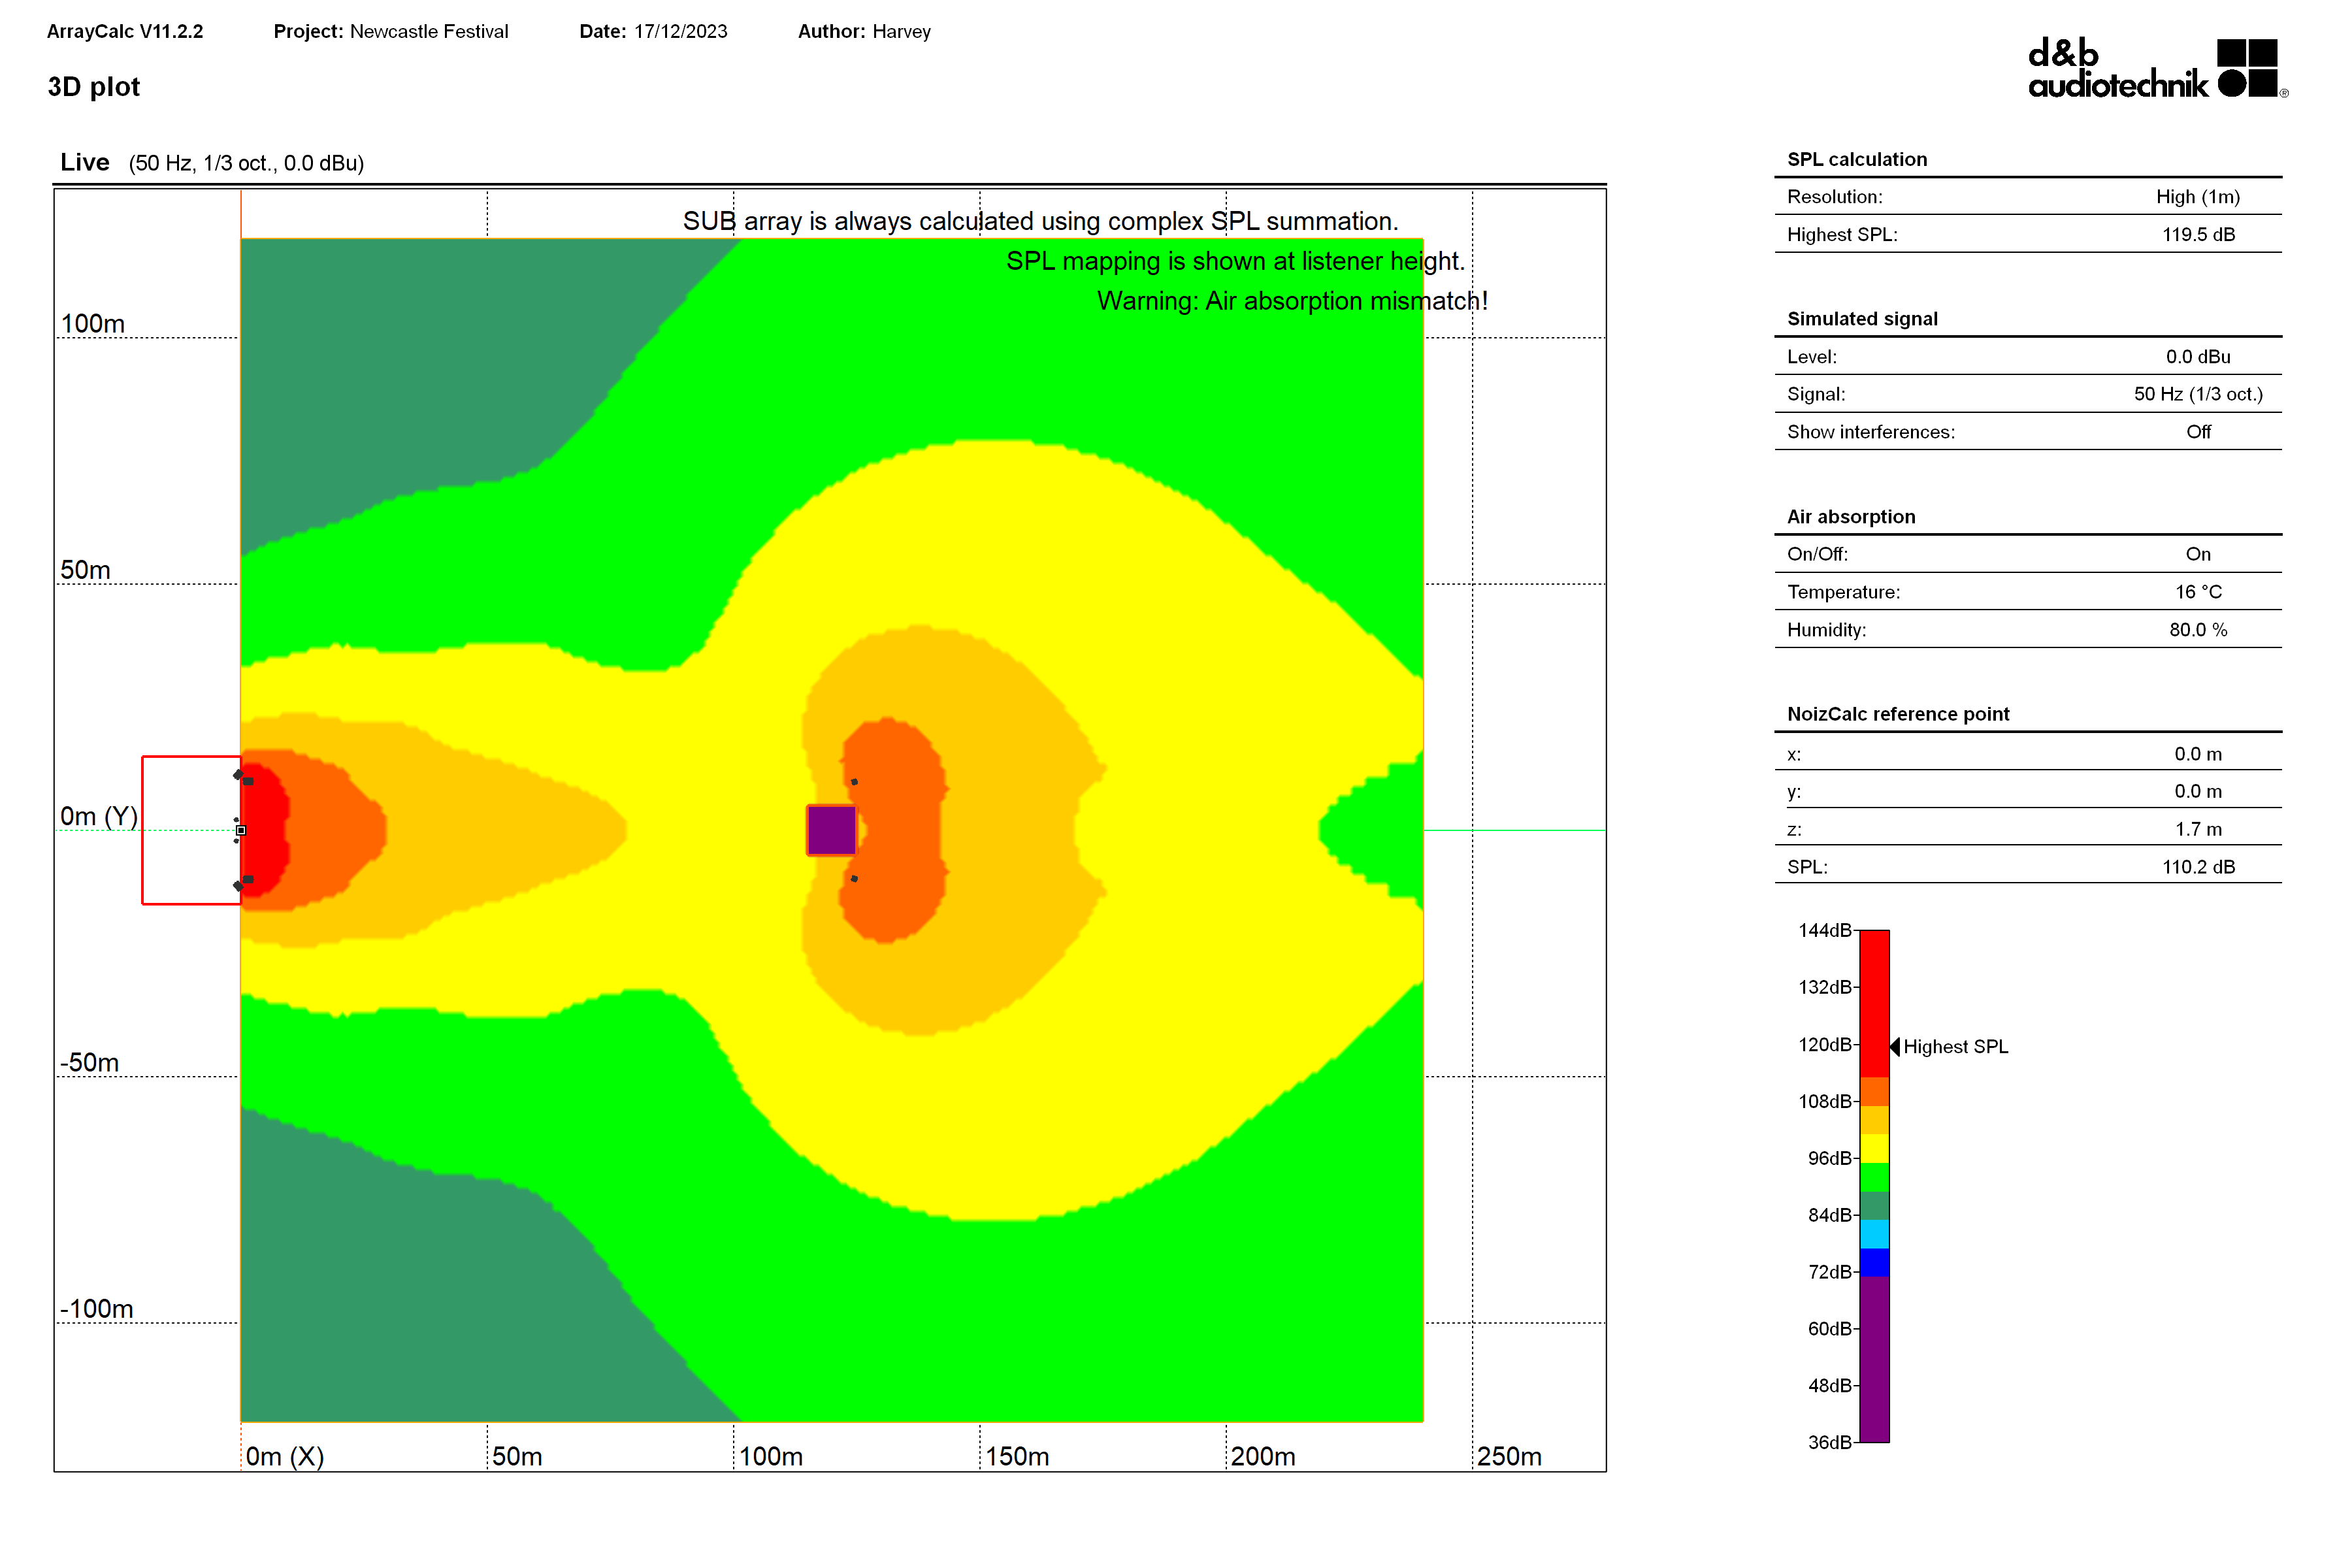
\includegraphics[width=0.5\textwidth]{Images/spl_plot_50hz_subs.png}}  & \multicolumn{1}{c|}{\SI{119.5}{\dB}} & \multicolumn{1}{c|}{\SI{84}{\dB}}  & \multicolumn{1}{c|}{\SI{25.1}{\dB}} & \SI{101.8}{\dB} \\ \hline
            \multicolumn{1}{|c|}{\SI{100}{\Hz}} & \multicolumn{1}{c|}{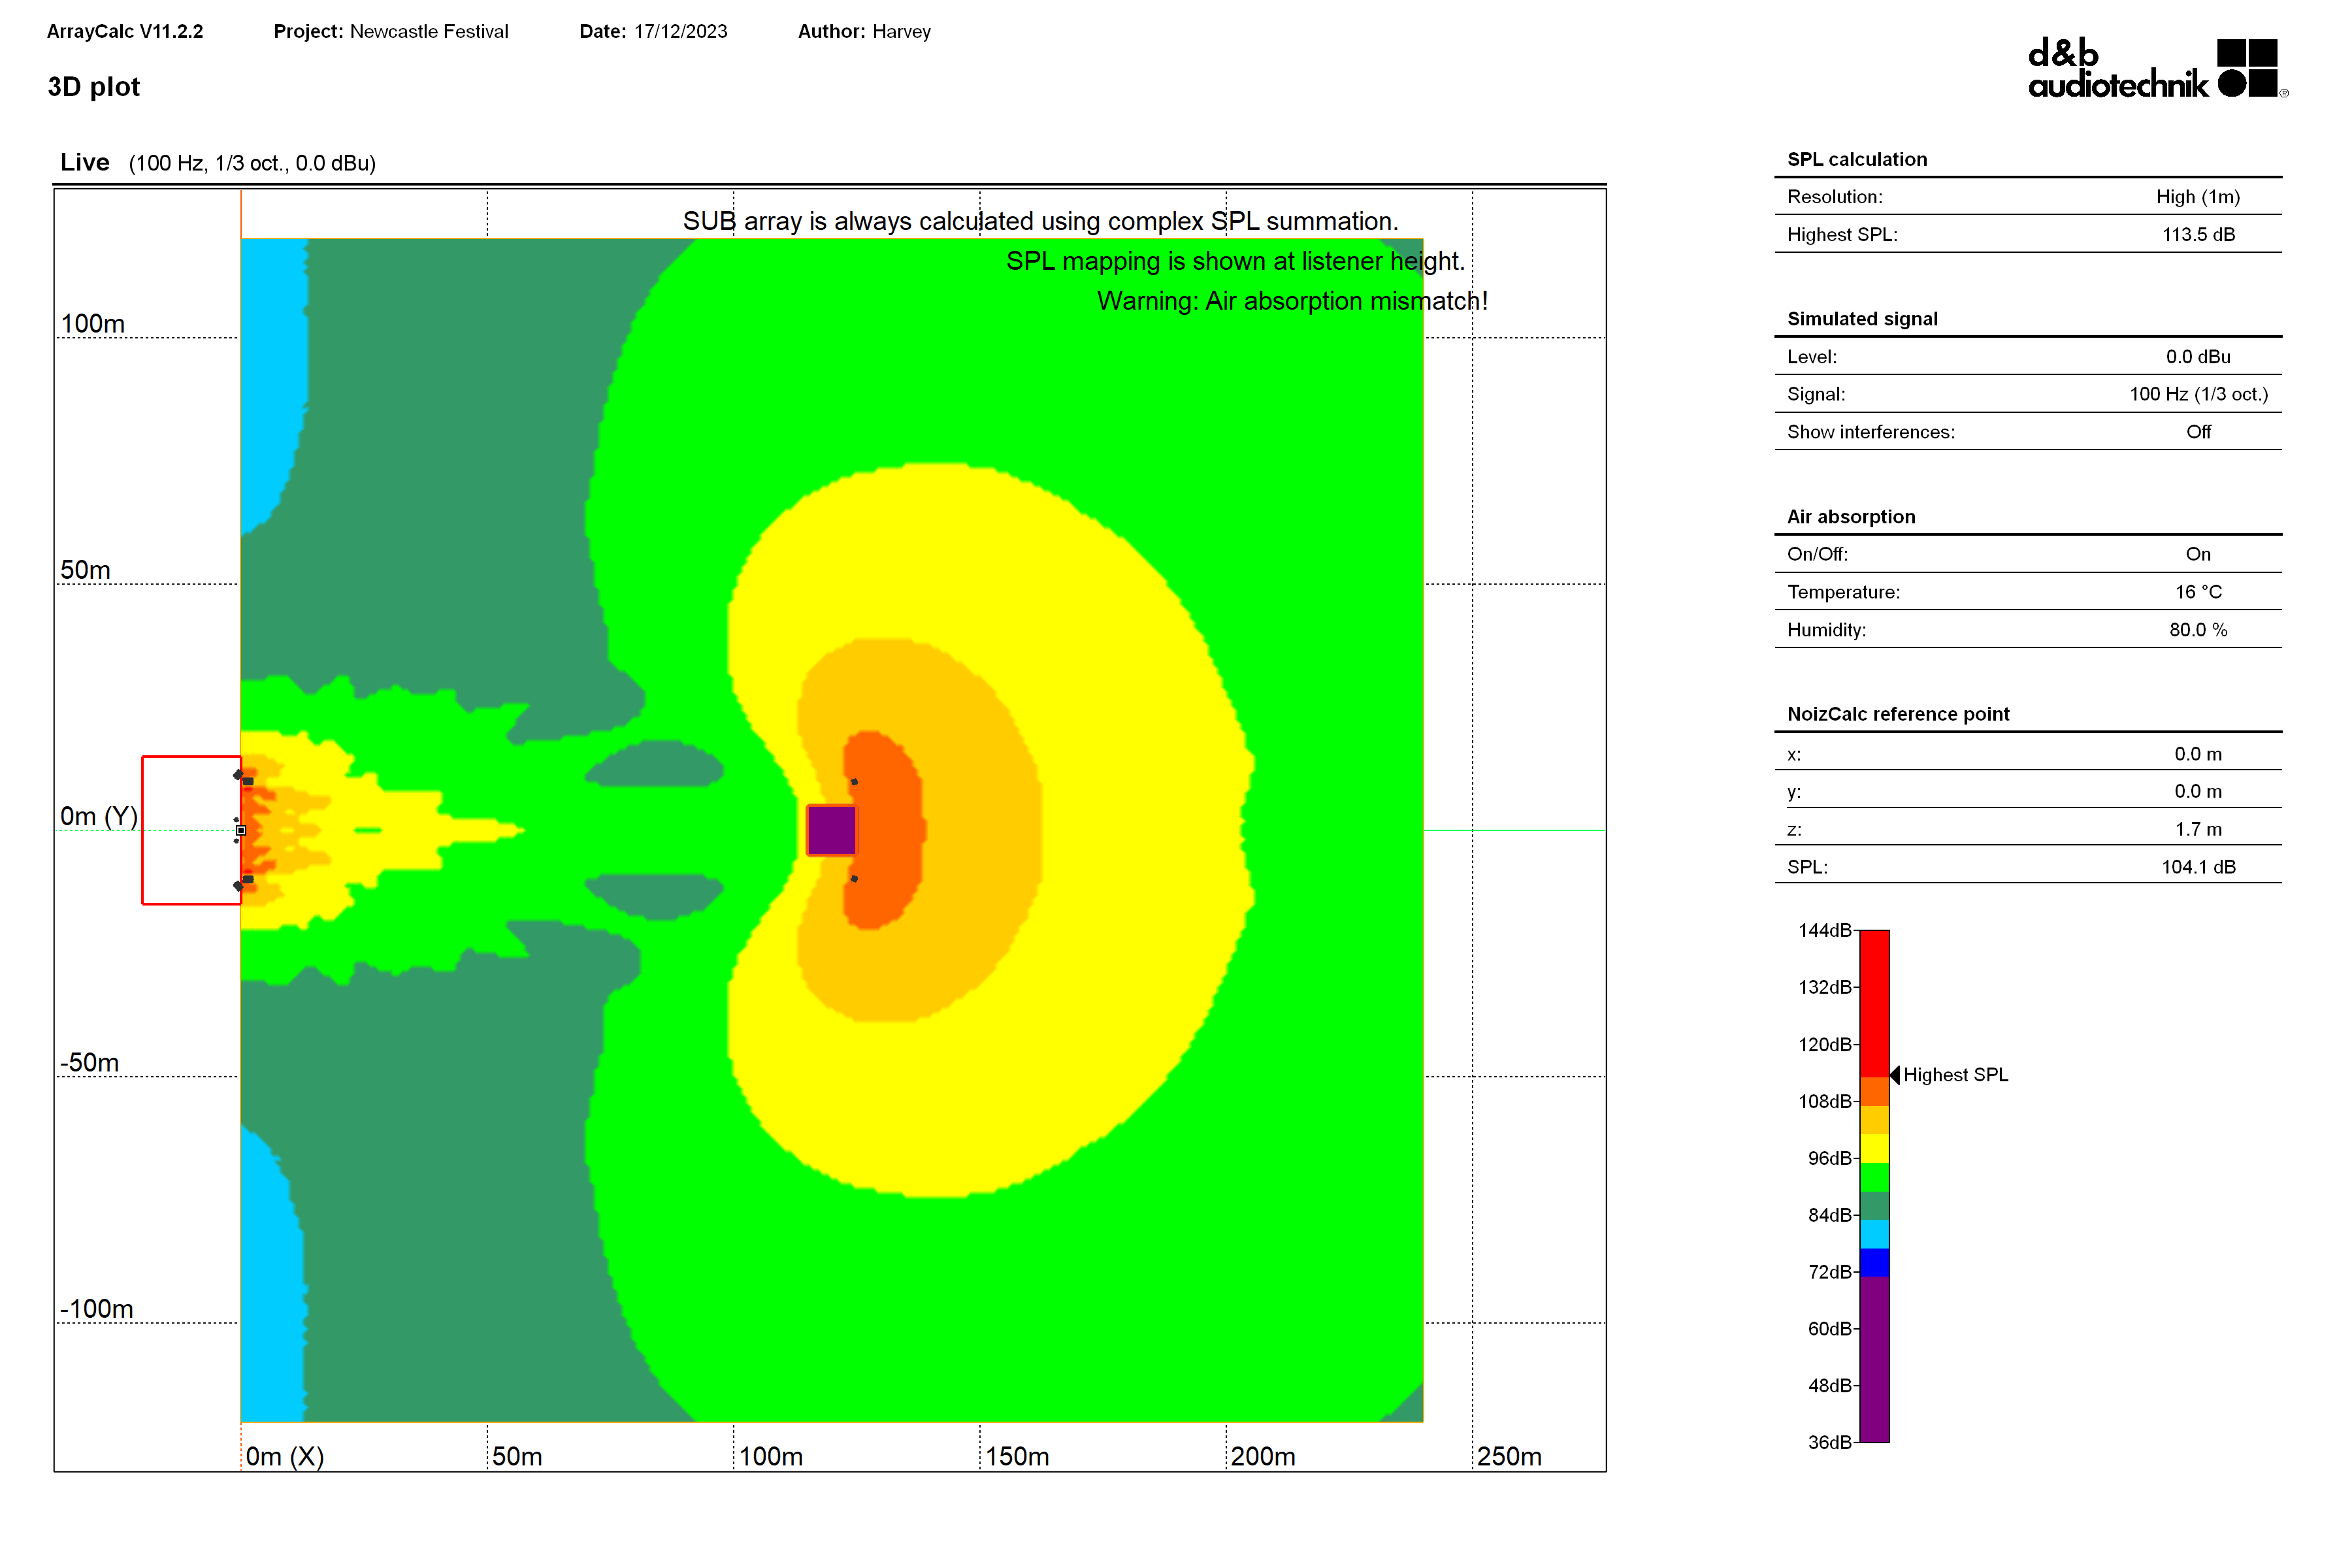
\includegraphics[width=0.5\textwidth]{Images/spl_plot_100hz_subs.png}} & \multicolumn{1}{c|}{\SI{113.5}{\dB}} & \multicolumn{1}{c|}{\SI{78}{\dB}}  & \multicolumn{1}{c|}{\SI{25.1}{\dB}} & \SI{95.8}{\dB} \\ \hline
            \multicolumn{6}{|c|}{\textbf{Full System}}                                                                                                        \\ \hline
            \multicolumn{1}{|c|}{\SI{50}{\Hz}}  & \multicolumn{1}{c|}{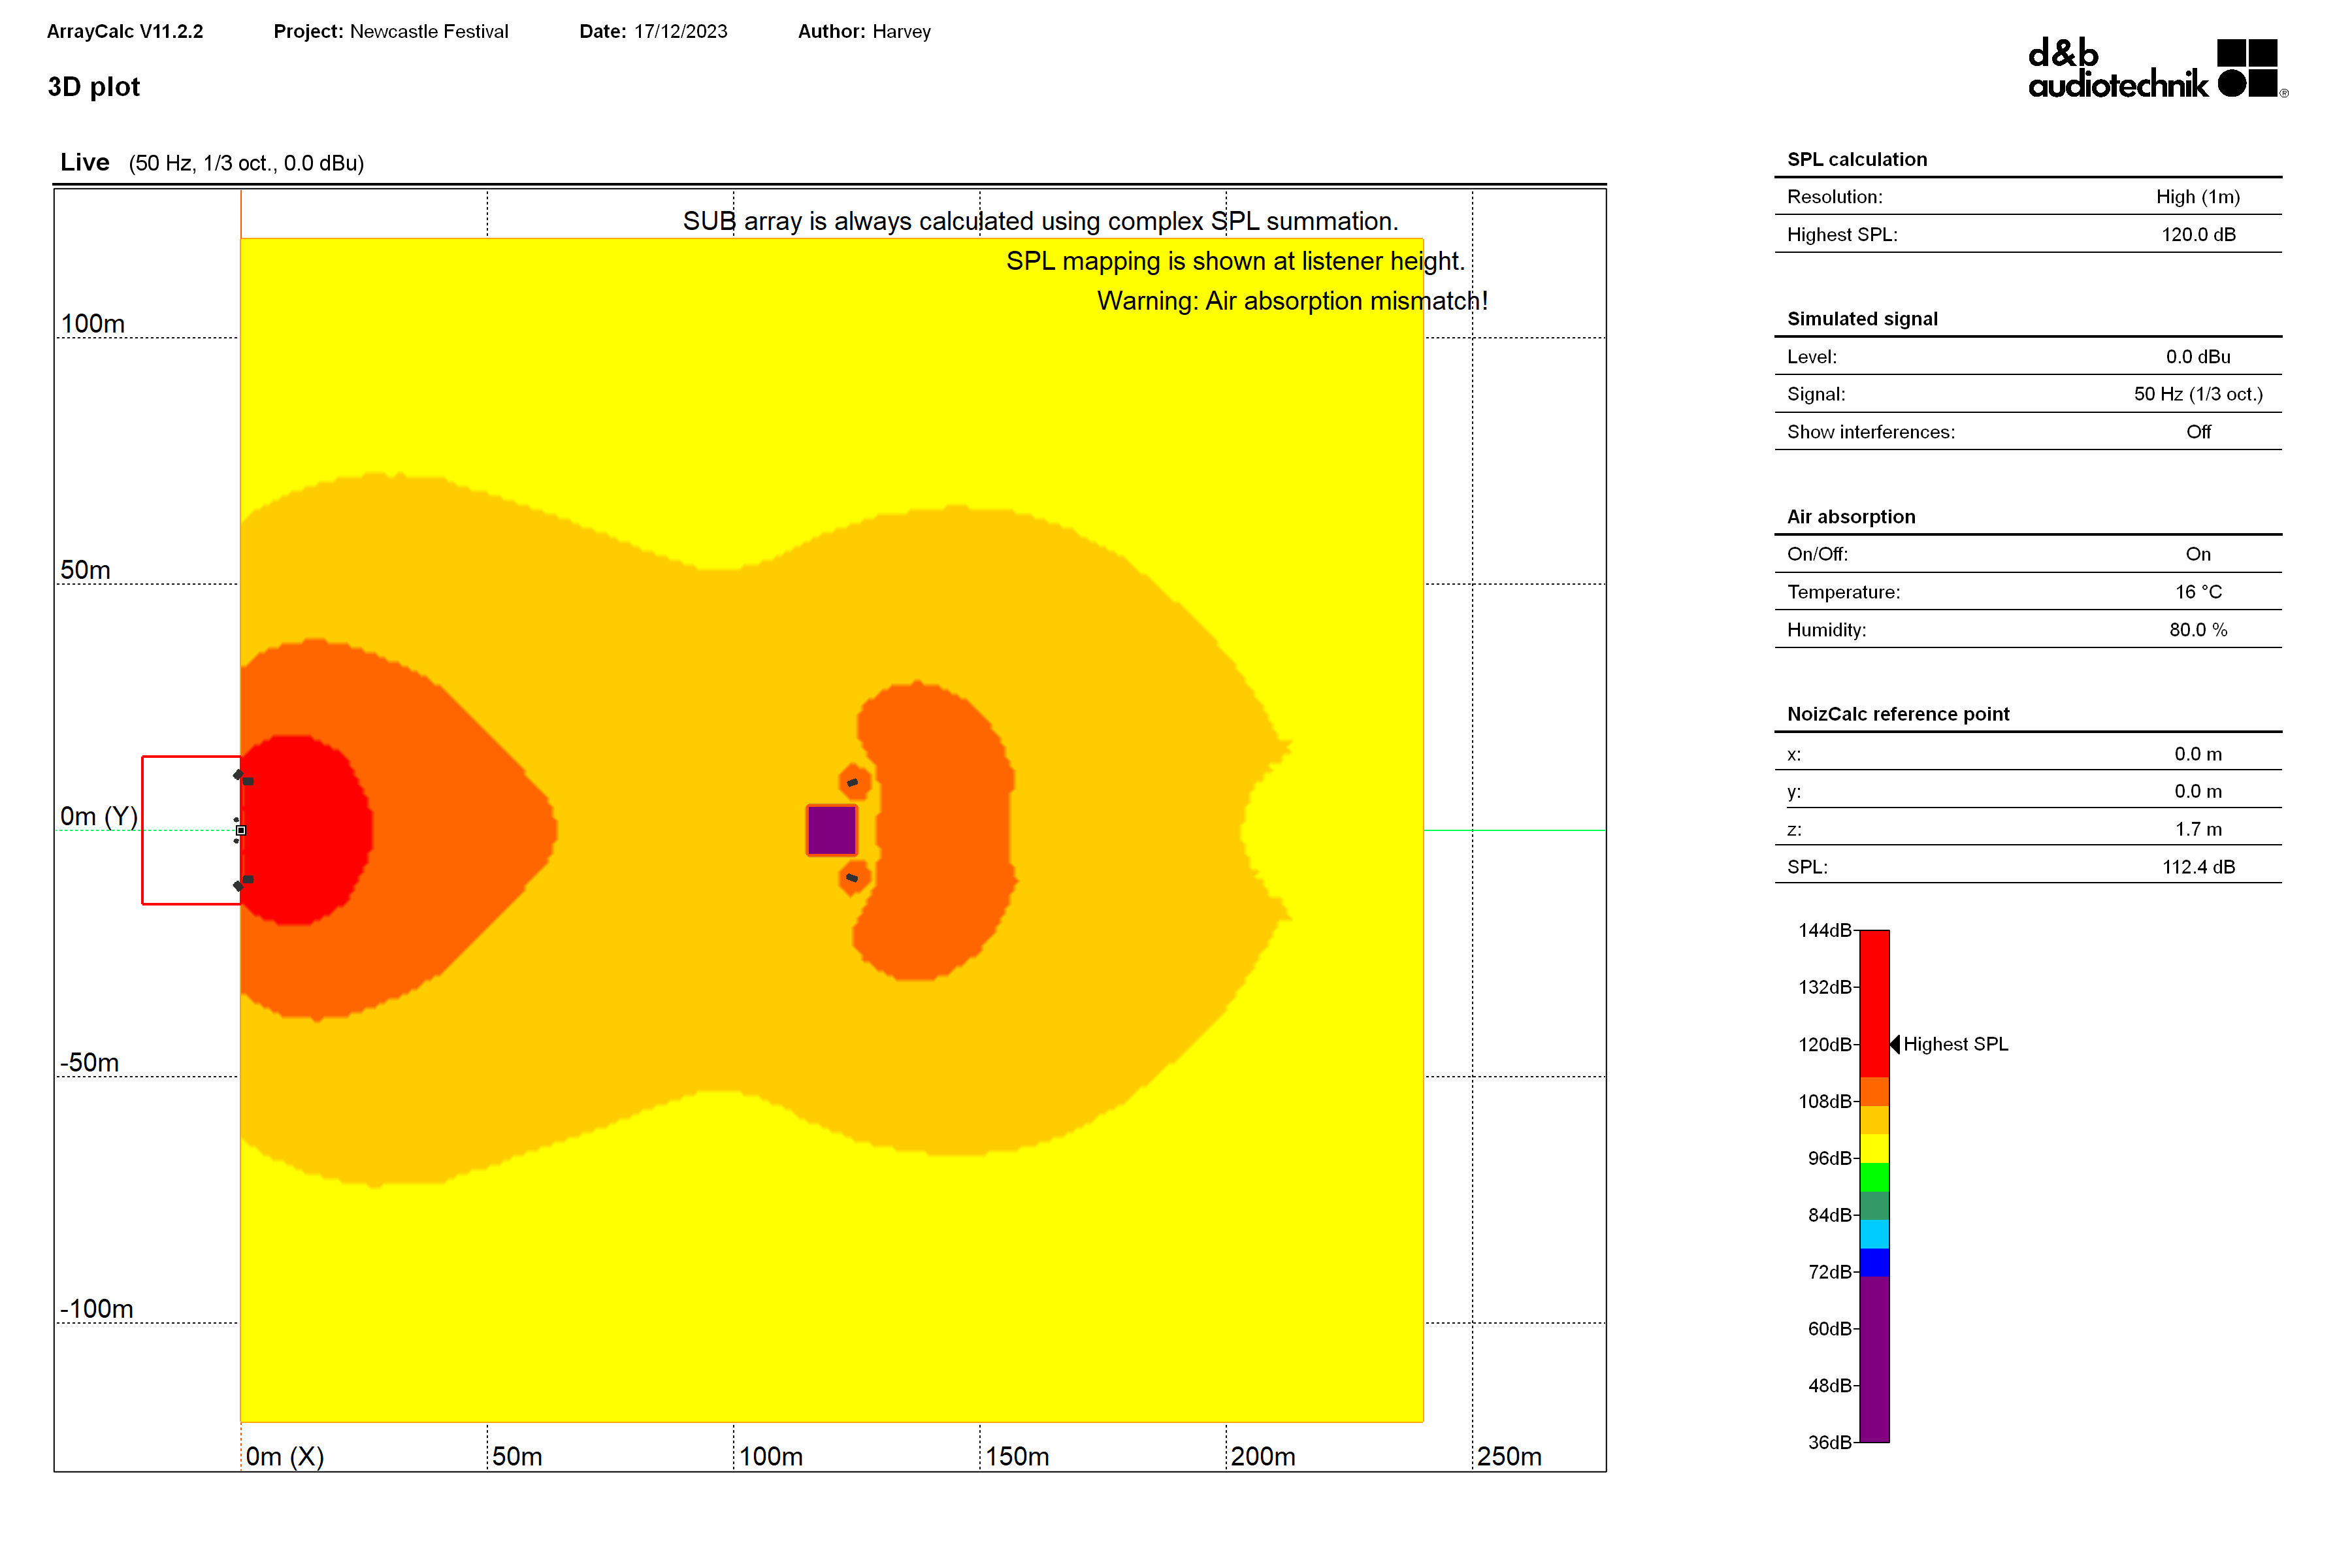
\includegraphics[width=0.5\textwidth]{Images/spl_plot_50hz_all.png}}   & \multicolumn{1}{c|}{\SI{120.0}{\dB}} & \multicolumn{1}{c|}{\SI{96}{\dB}}  & \multicolumn{1}{c|}{\SI{17.0}{\dB}} & \SI{108.0}{\dB} \\ \hline
            \multicolumn{1}{|c|}{\SI{100}{\Hz}} & \multicolumn{1}{c|}{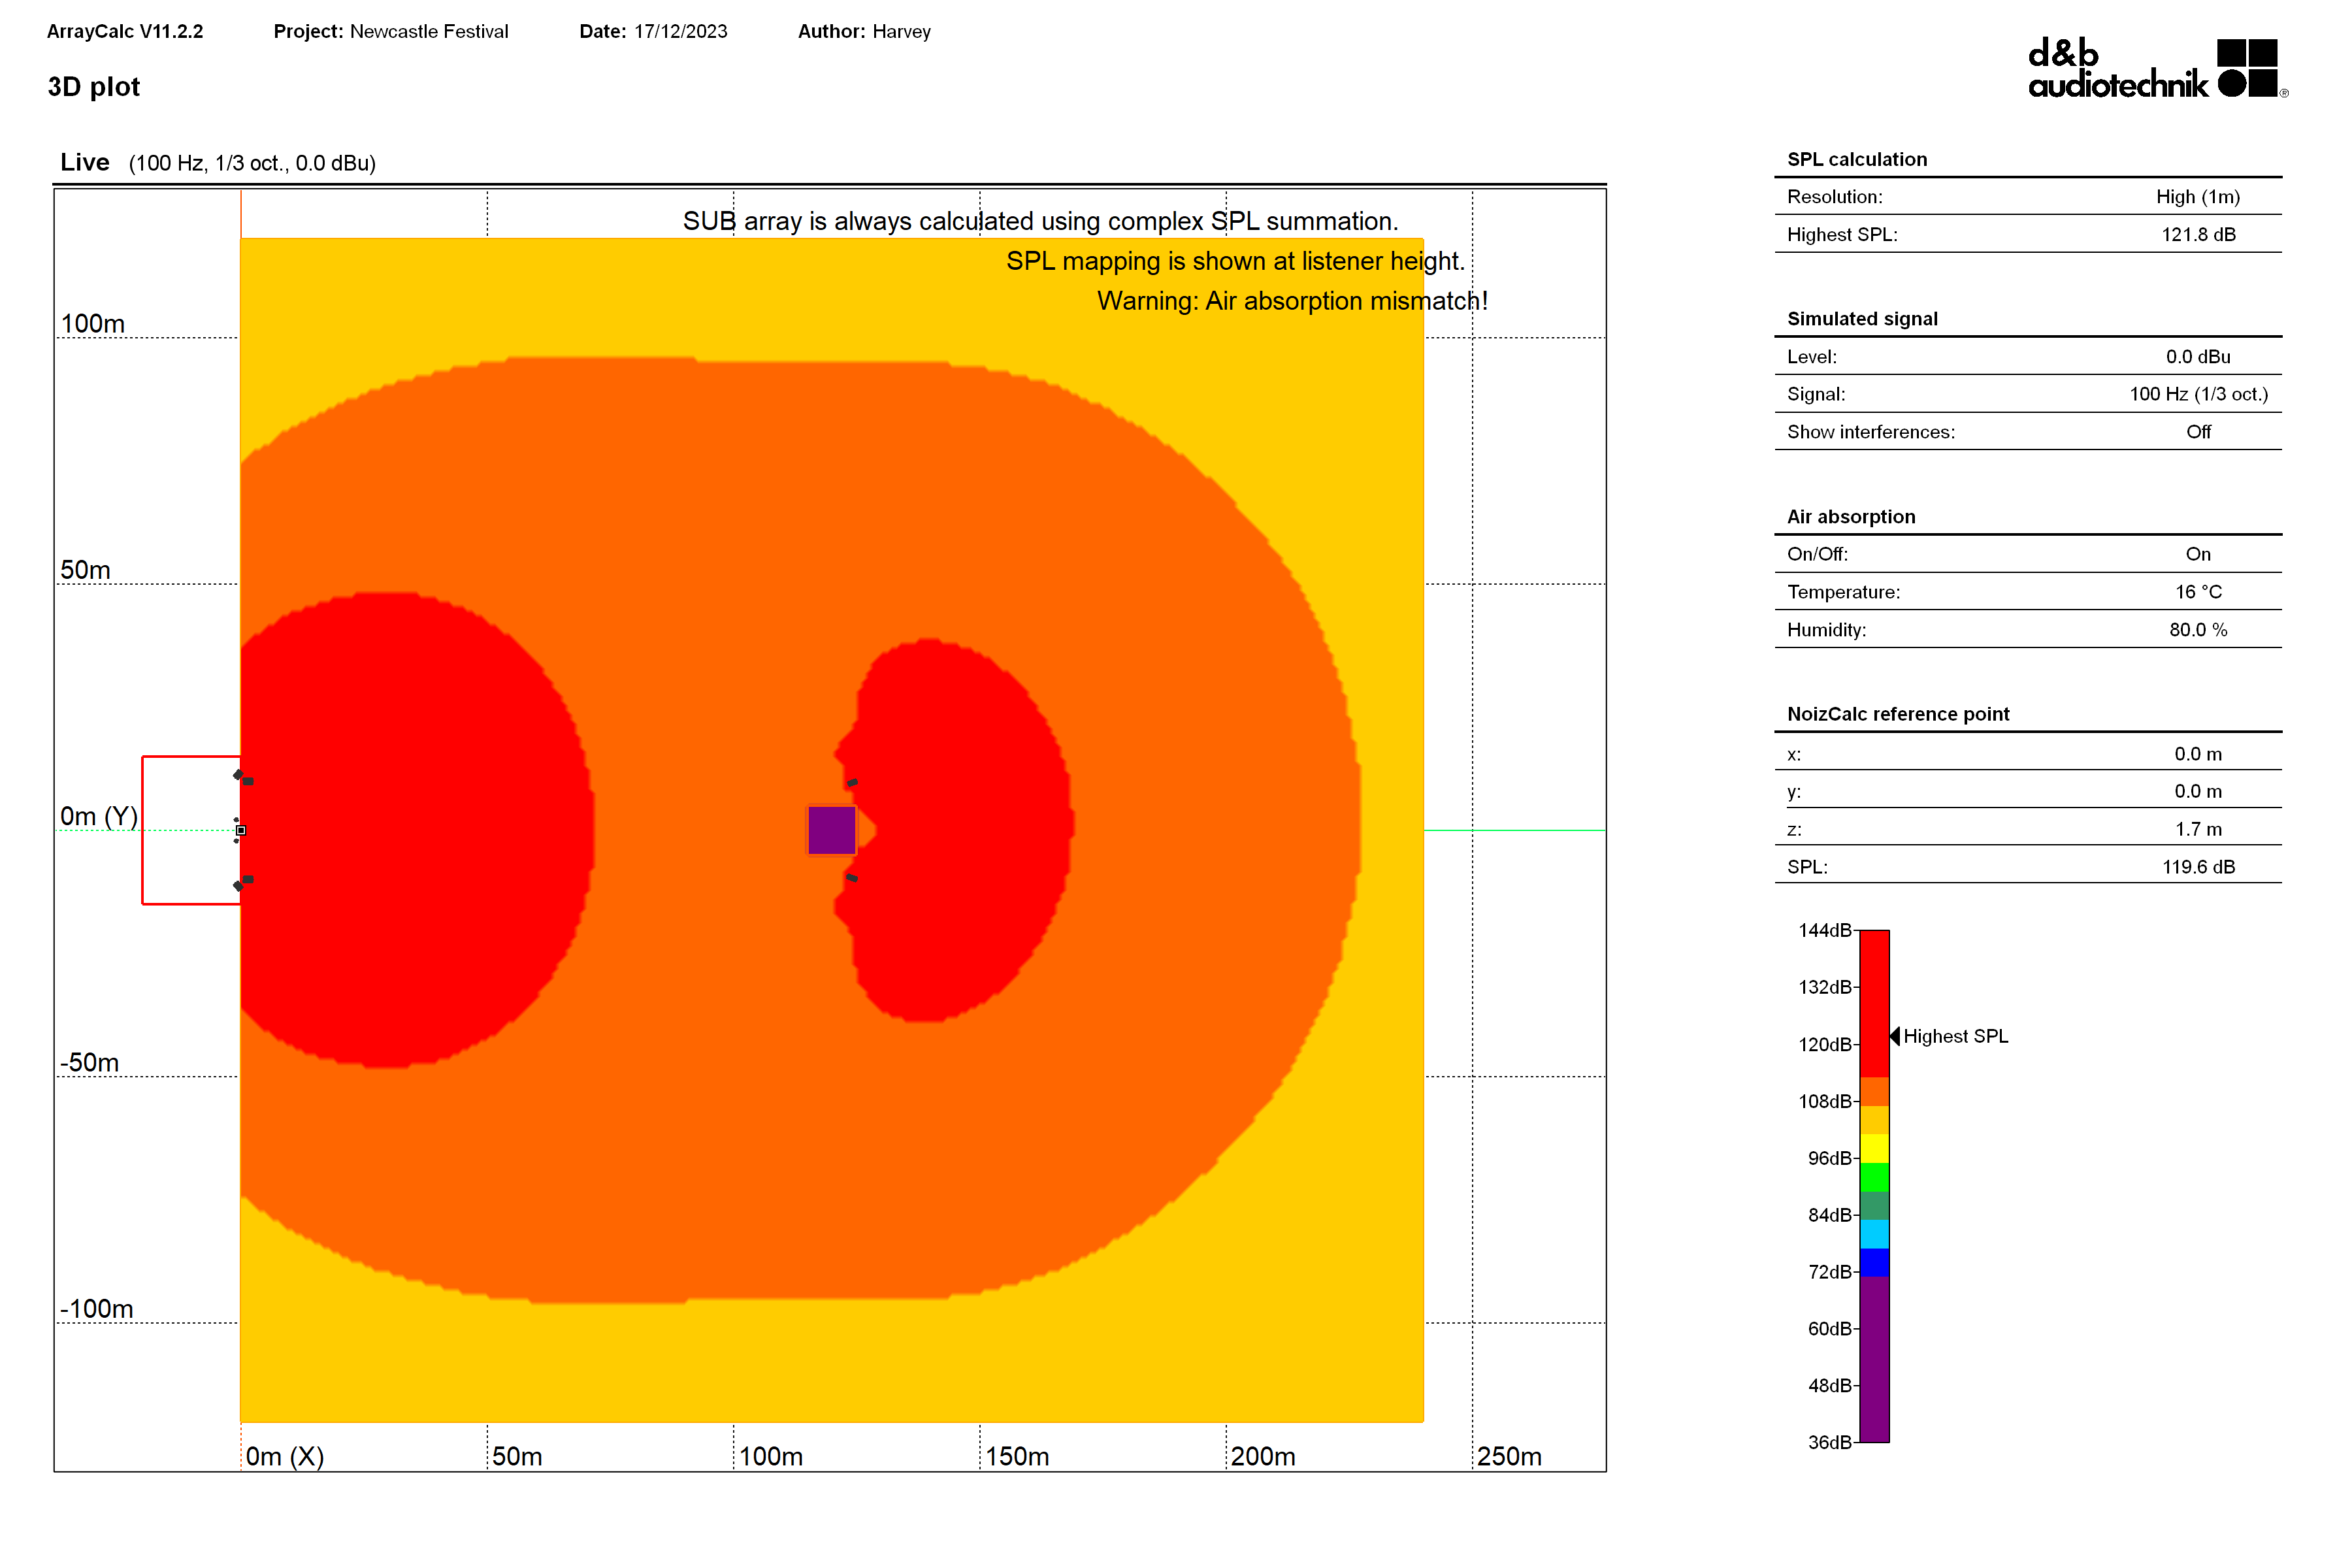
\includegraphics[width=0.5\textwidth]{Images/spl_plot_100hz_all.png}}  & \multicolumn{1}{c|}{\SI{121.8}{\dB}} & \multicolumn{1}{c|}{\SI{102}{\dB}} & \multicolumn{1}{c|}{\SI{14.0}{\dB}} & \SI{111.9}{\dB} \\ \hline
            \multicolumn{1}{|c|}{\SI{500}{\Hz}} & \multicolumn{1}{c|}{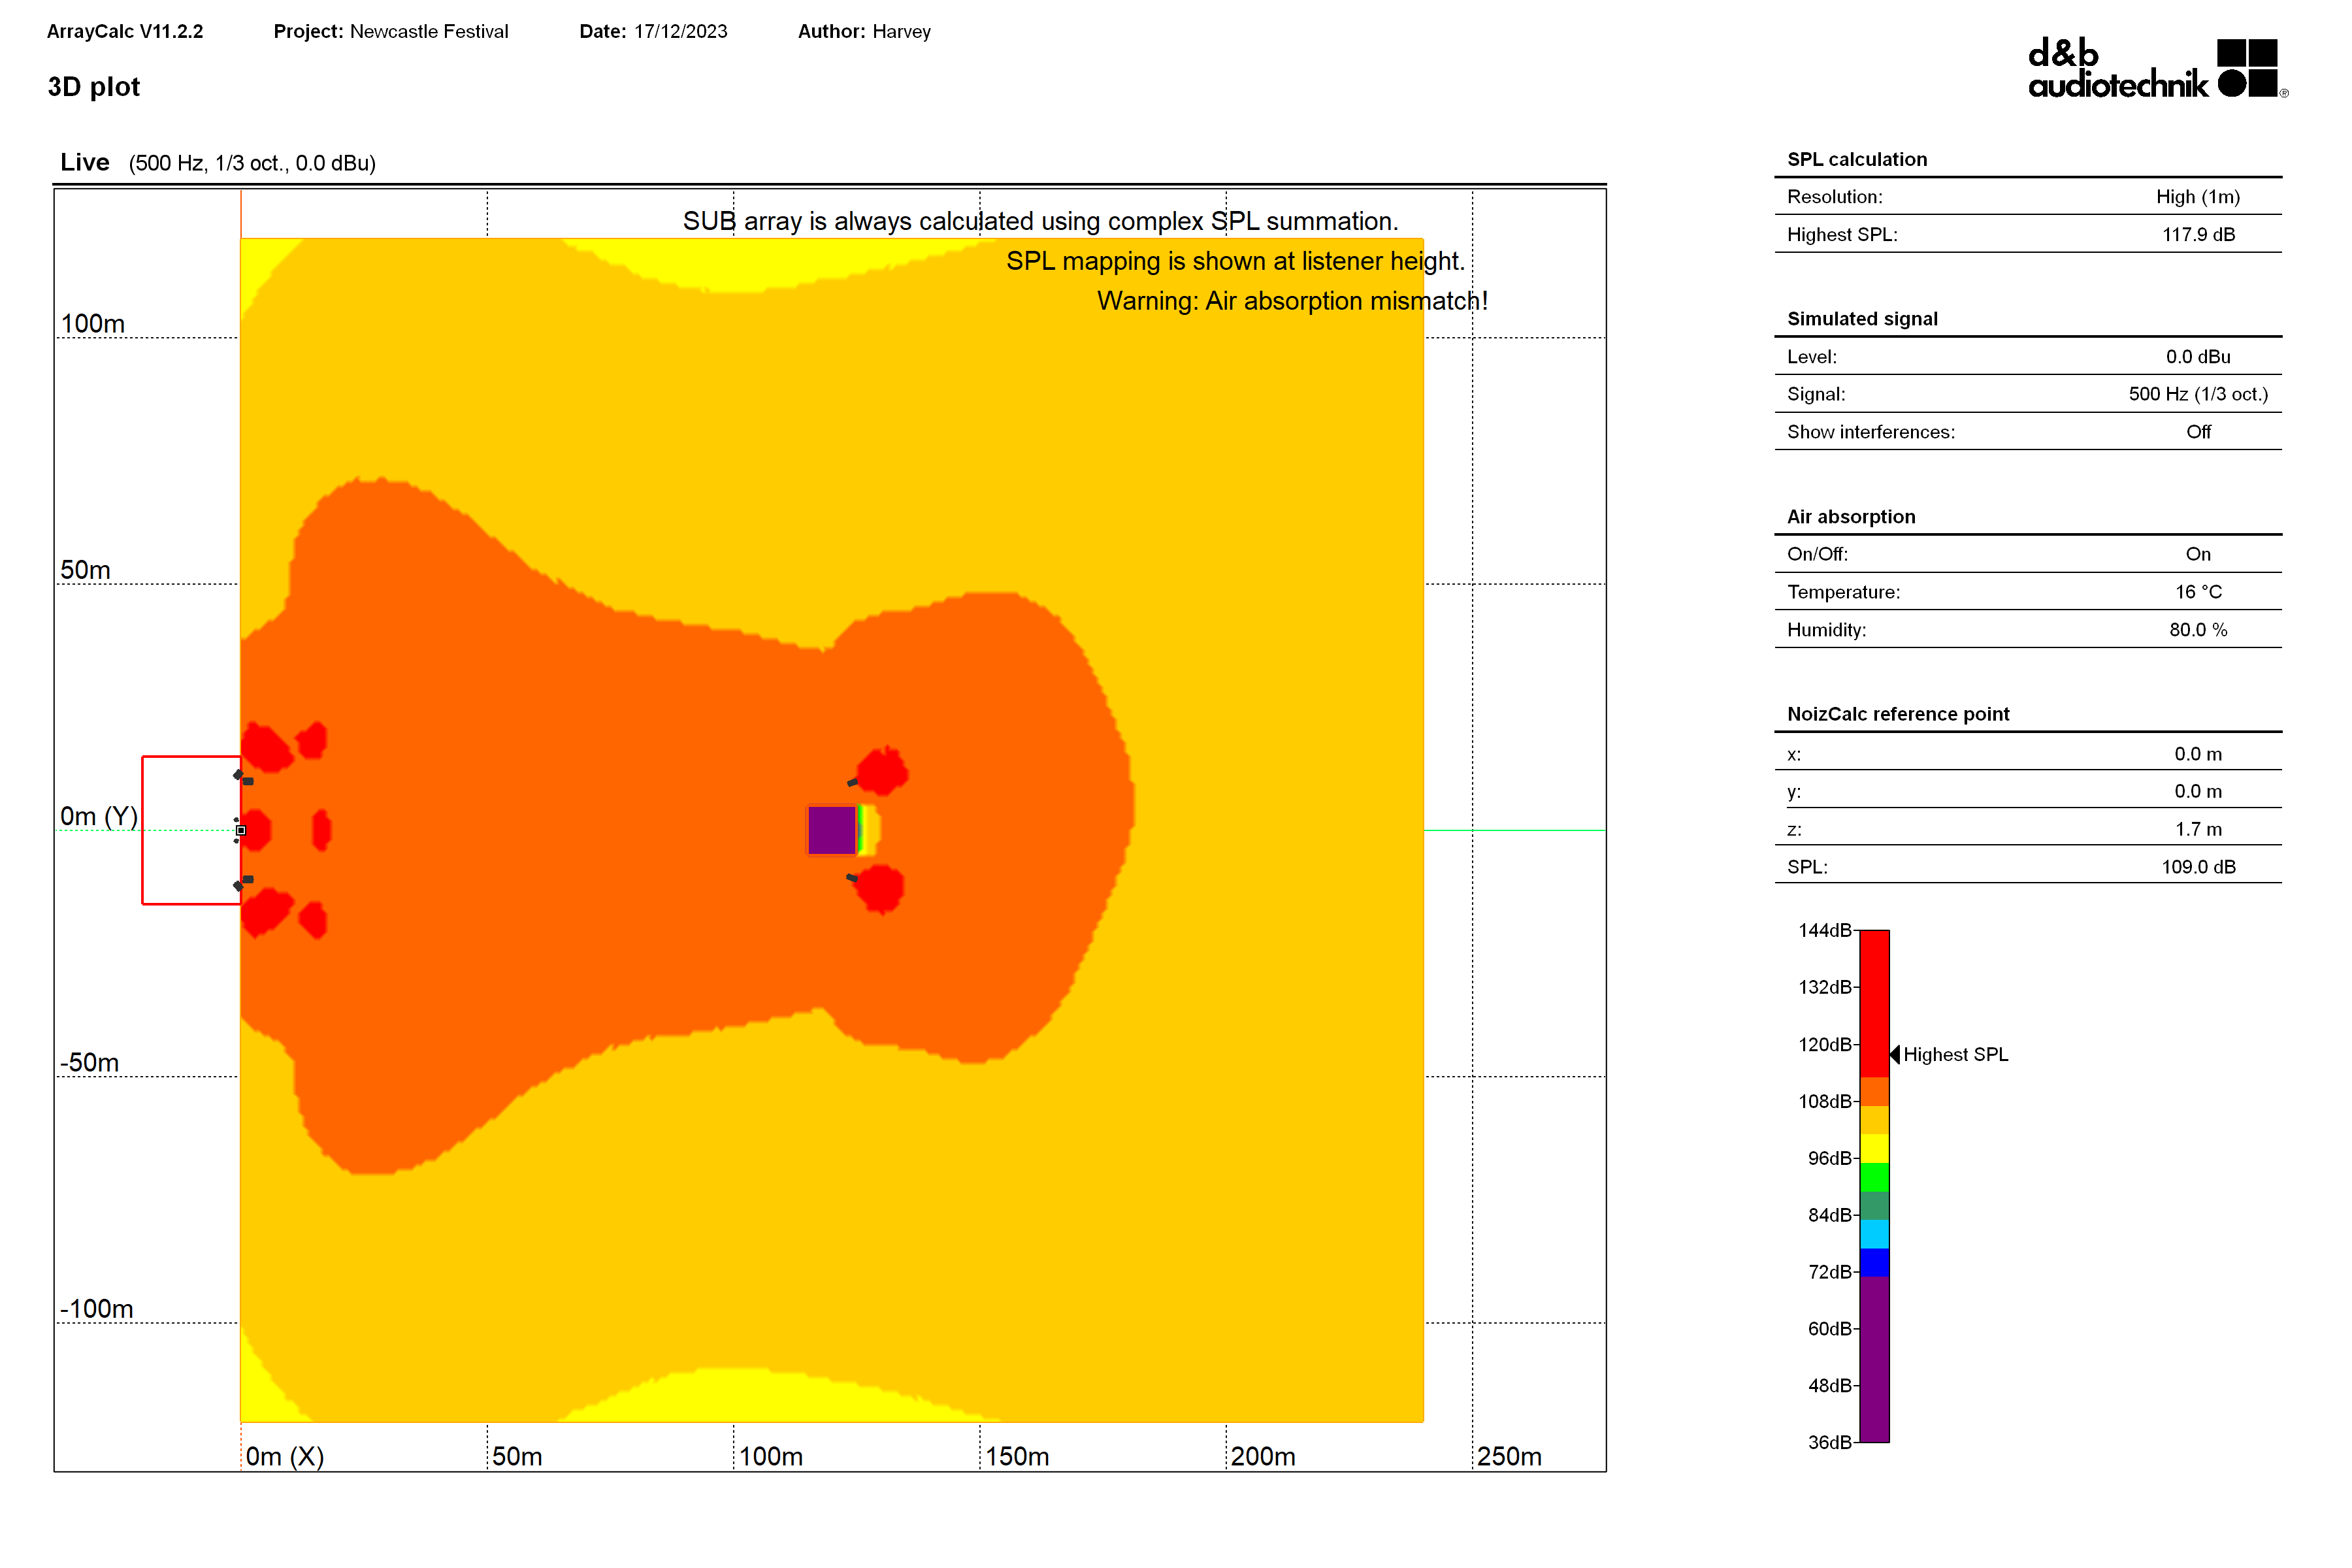
\includegraphics[width=0.5\textwidth]{Images/spl_plot_500hz.png}}      & \multicolumn{1}{c|}{\SI{117.9}{\dB}} & \multicolumn{1}{c|}{\SI{96}{\dB}}  & \multicolumn{1}{c|}{\SI{15.5}{\dB}} & \SI{107.0}{\dB} \\ \hline
            \multicolumn{1}{|c|}{\SI{1}{\kHz}}  & \multicolumn{1}{c|}{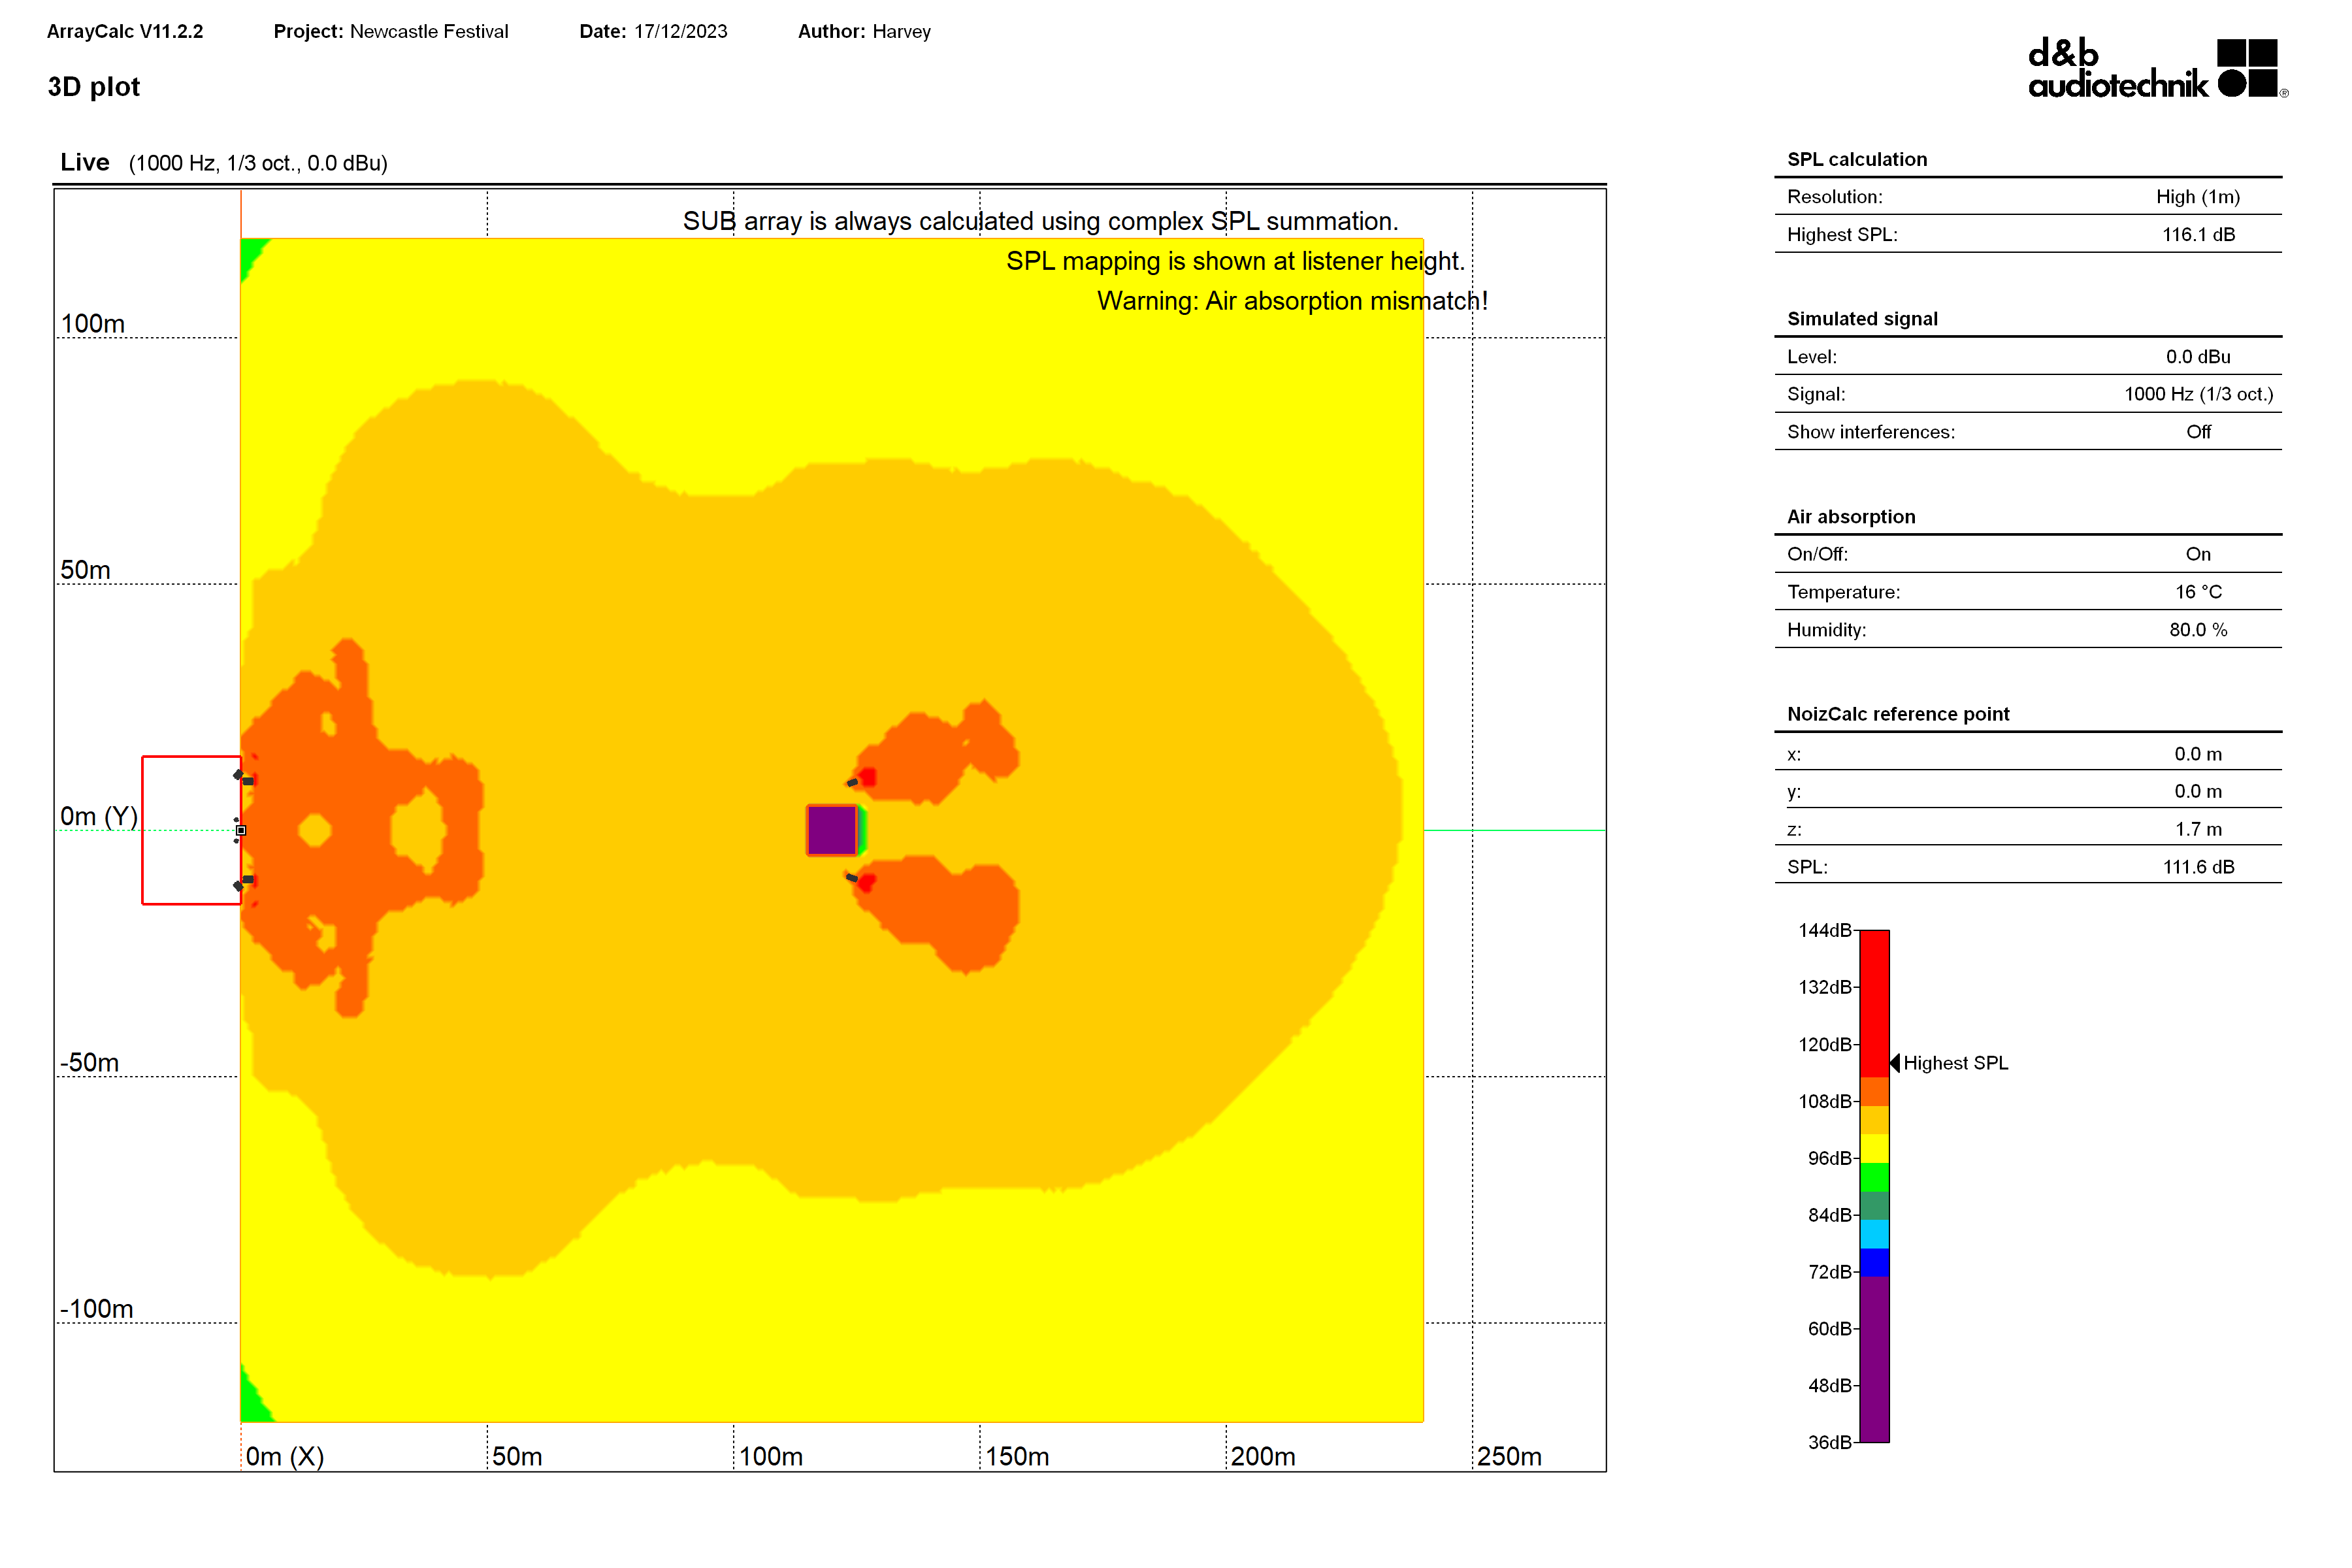
\includegraphics[width=0.5\textwidth]{Images/spl_plot_1khz.png}}       & \multicolumn{1}{c|}{\SI{116.1}{\dB}} & \multicolumn{1}{c|}{\SI{90}{\dB}}  & \multicolumn{1}{c|}{\SI{18.5}{\dB}} & \SI{103.1}{\dB} \\ \hline
            \multicolumn{1}{|c|}{\SI{2}{\kHz}}  & \multicolumn{1}{c|}{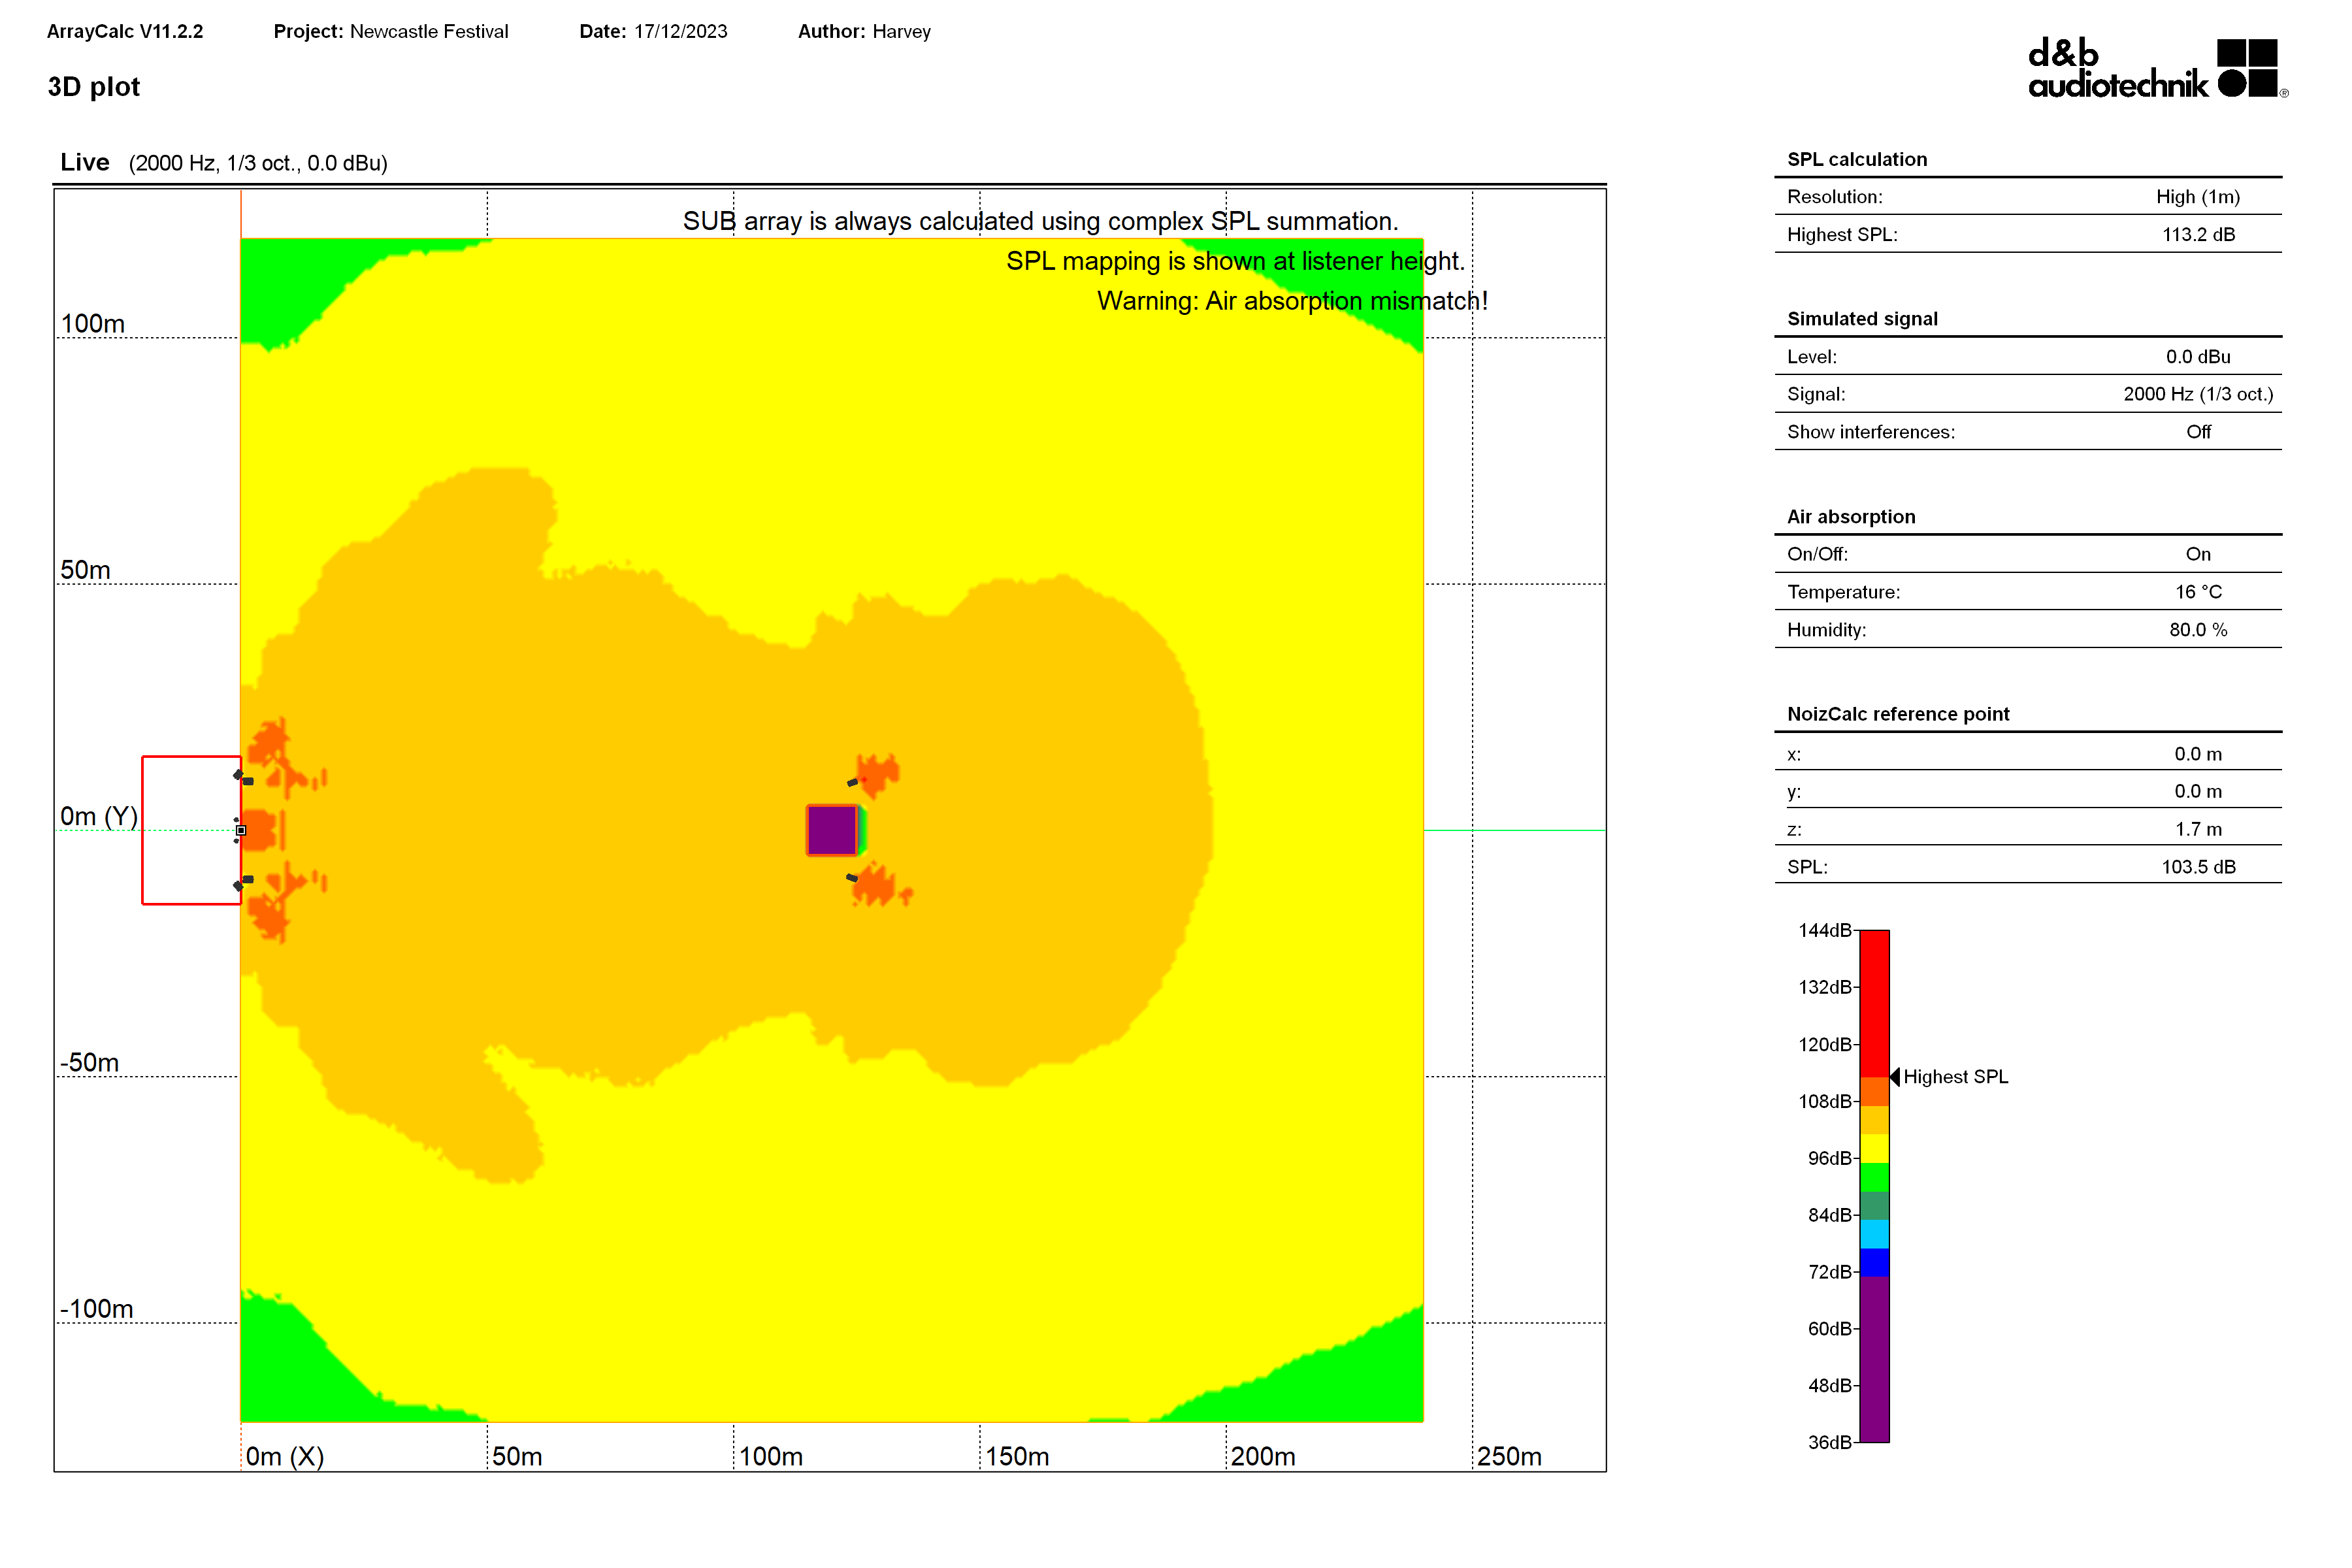
\includegraphics[width=0.5\textwidth]{Images/spl_plot_2khz.png}}       & \multicolumn{1}{c|}{\SI{116.1}{\dB}} & \multicolumn{1}{c|}{\SI{90}{\dB}}  & \multicolumn{1}{c|}{\SI{18.5}{\dB}} & \SI{103.1}{\dB} \\ \hline
            \multicolumn{1}{|c|}{\SI{5}{\kHz}}  & \multicolumn{1}{c|}{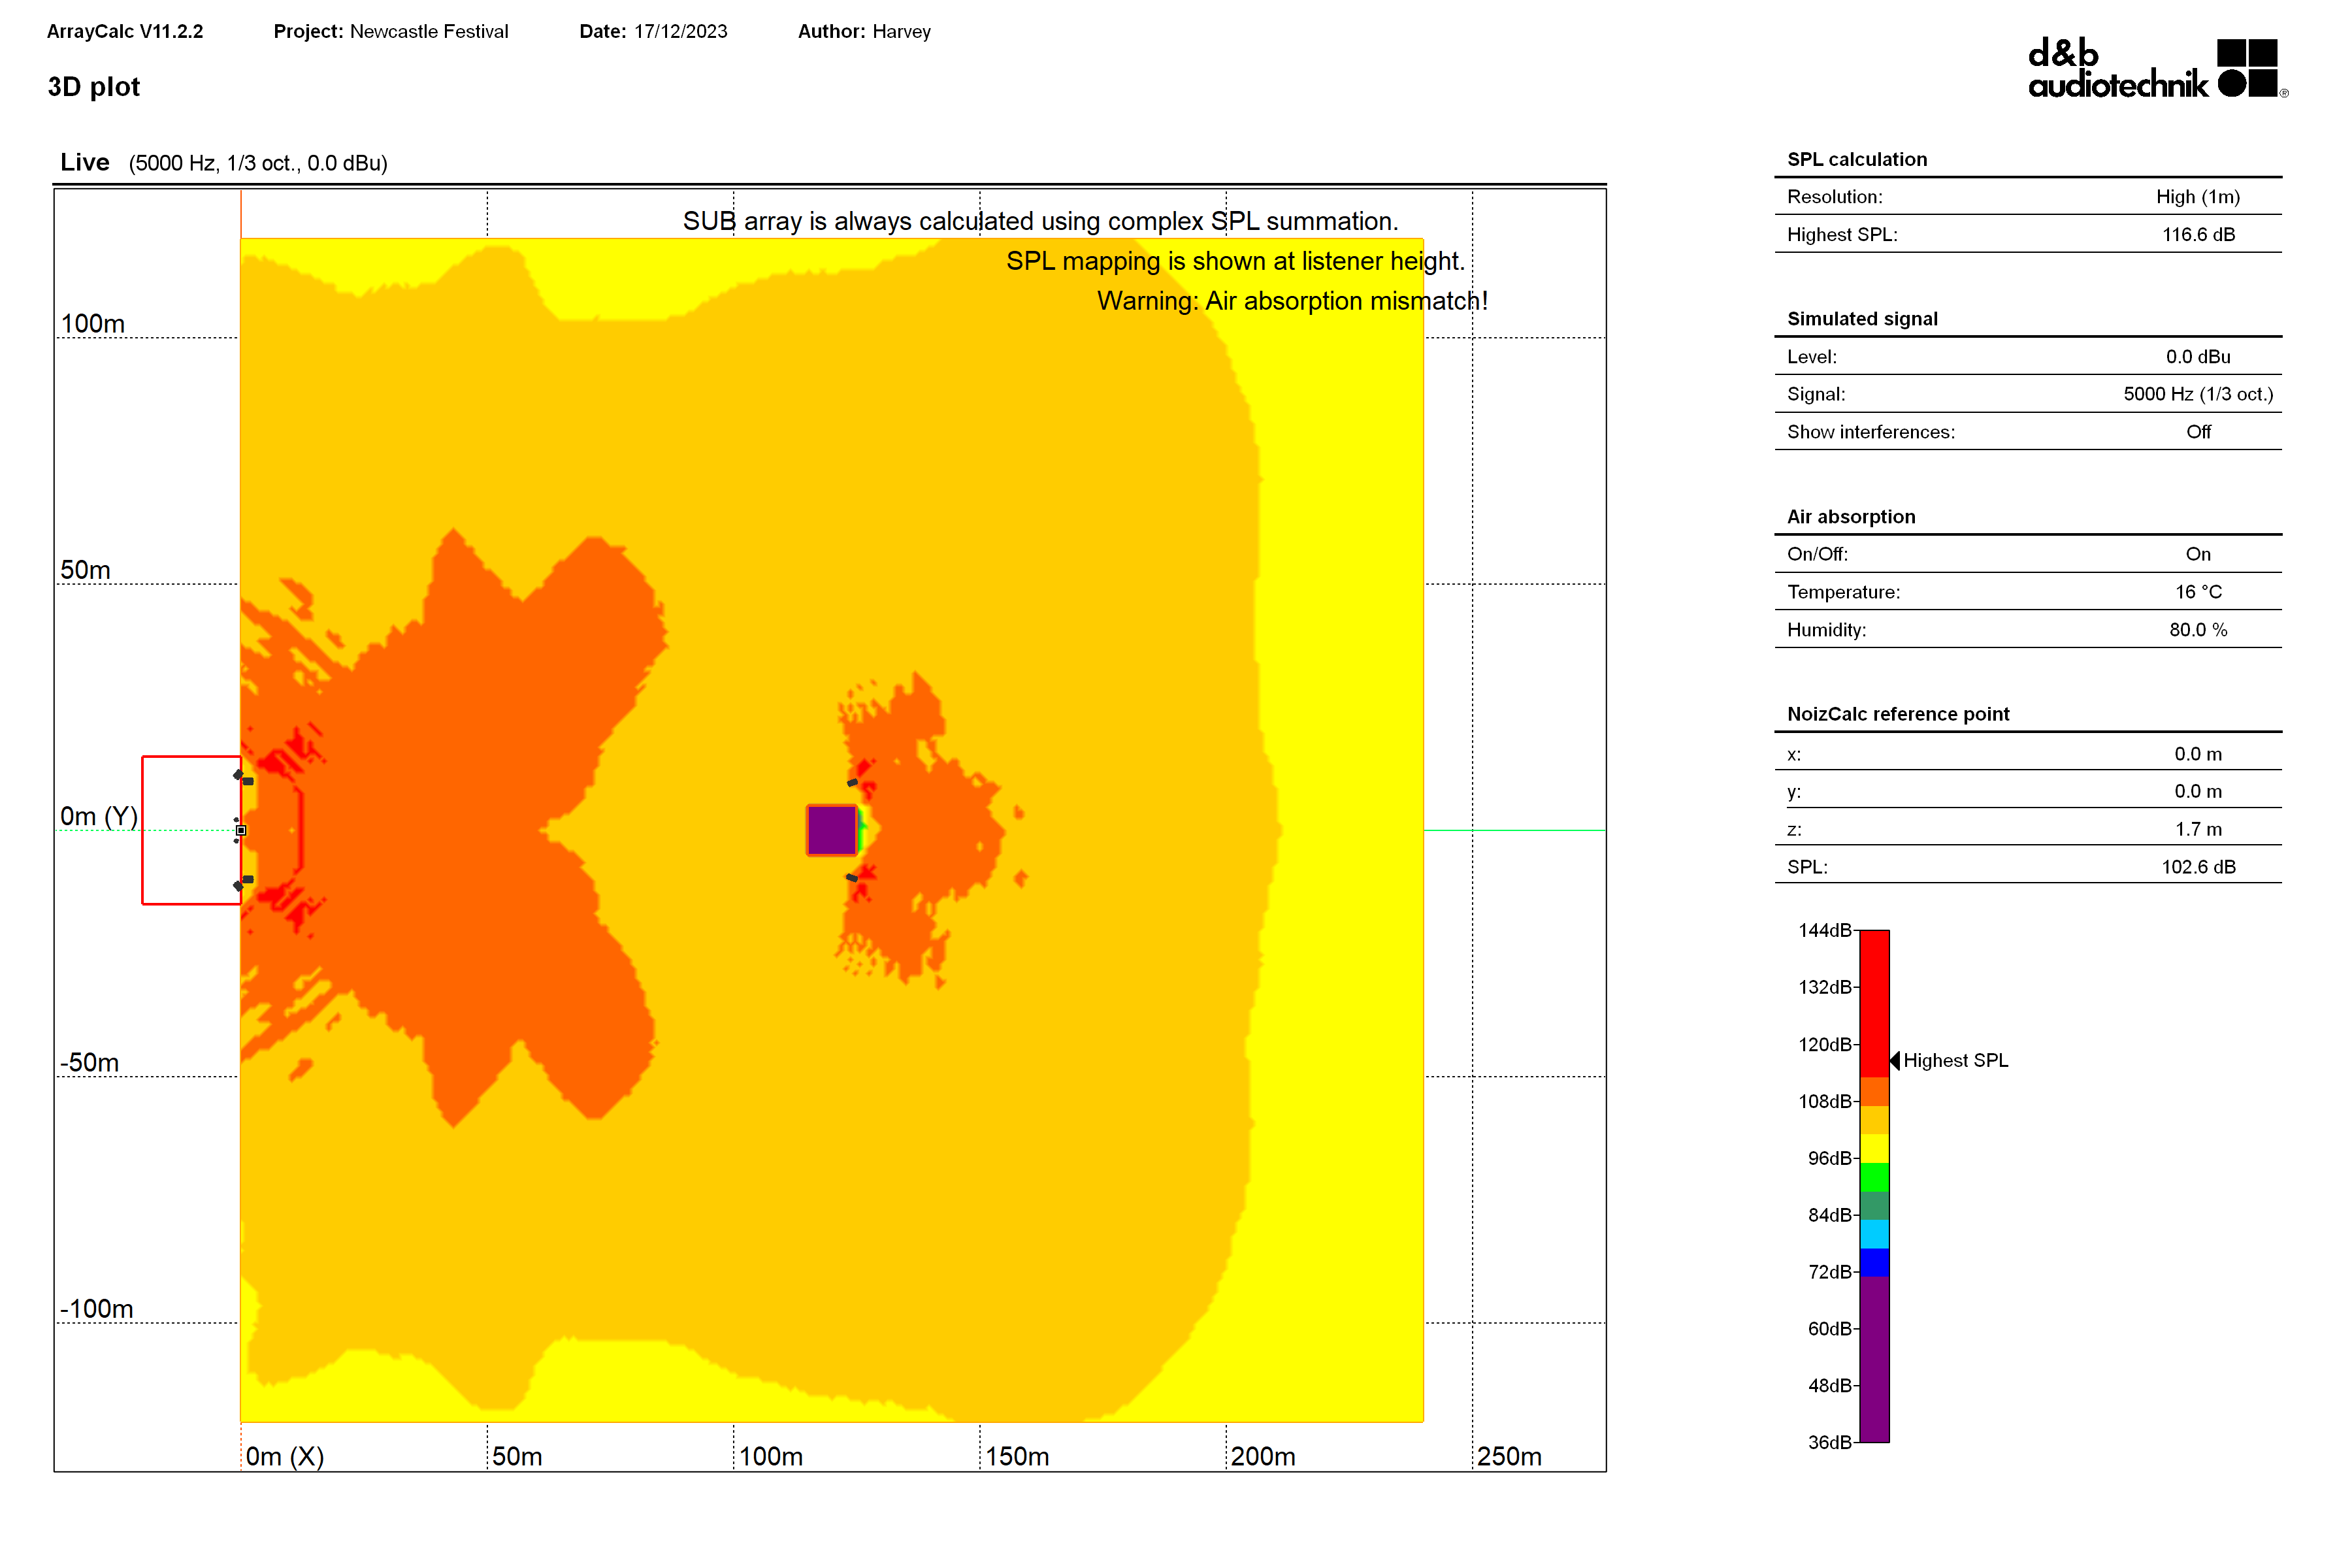
\includegraphics[width=0.5\textwidth]{Images/spl_plot_5khz.png}}       & \multicolumn{1}{c|}{\SI{116.6}{\dB}} & \multicolumn{1}{c|}{\SI{96}{\dB}}  & \multicolumn{1}{c|}{\SI{14.6}{\dB}} & \SI{106.3}{\dB} \\ \hline
            \multicolumn{1}{|c|}{\SI{10}{\kHz}} & \multicolumn{1}{c|}{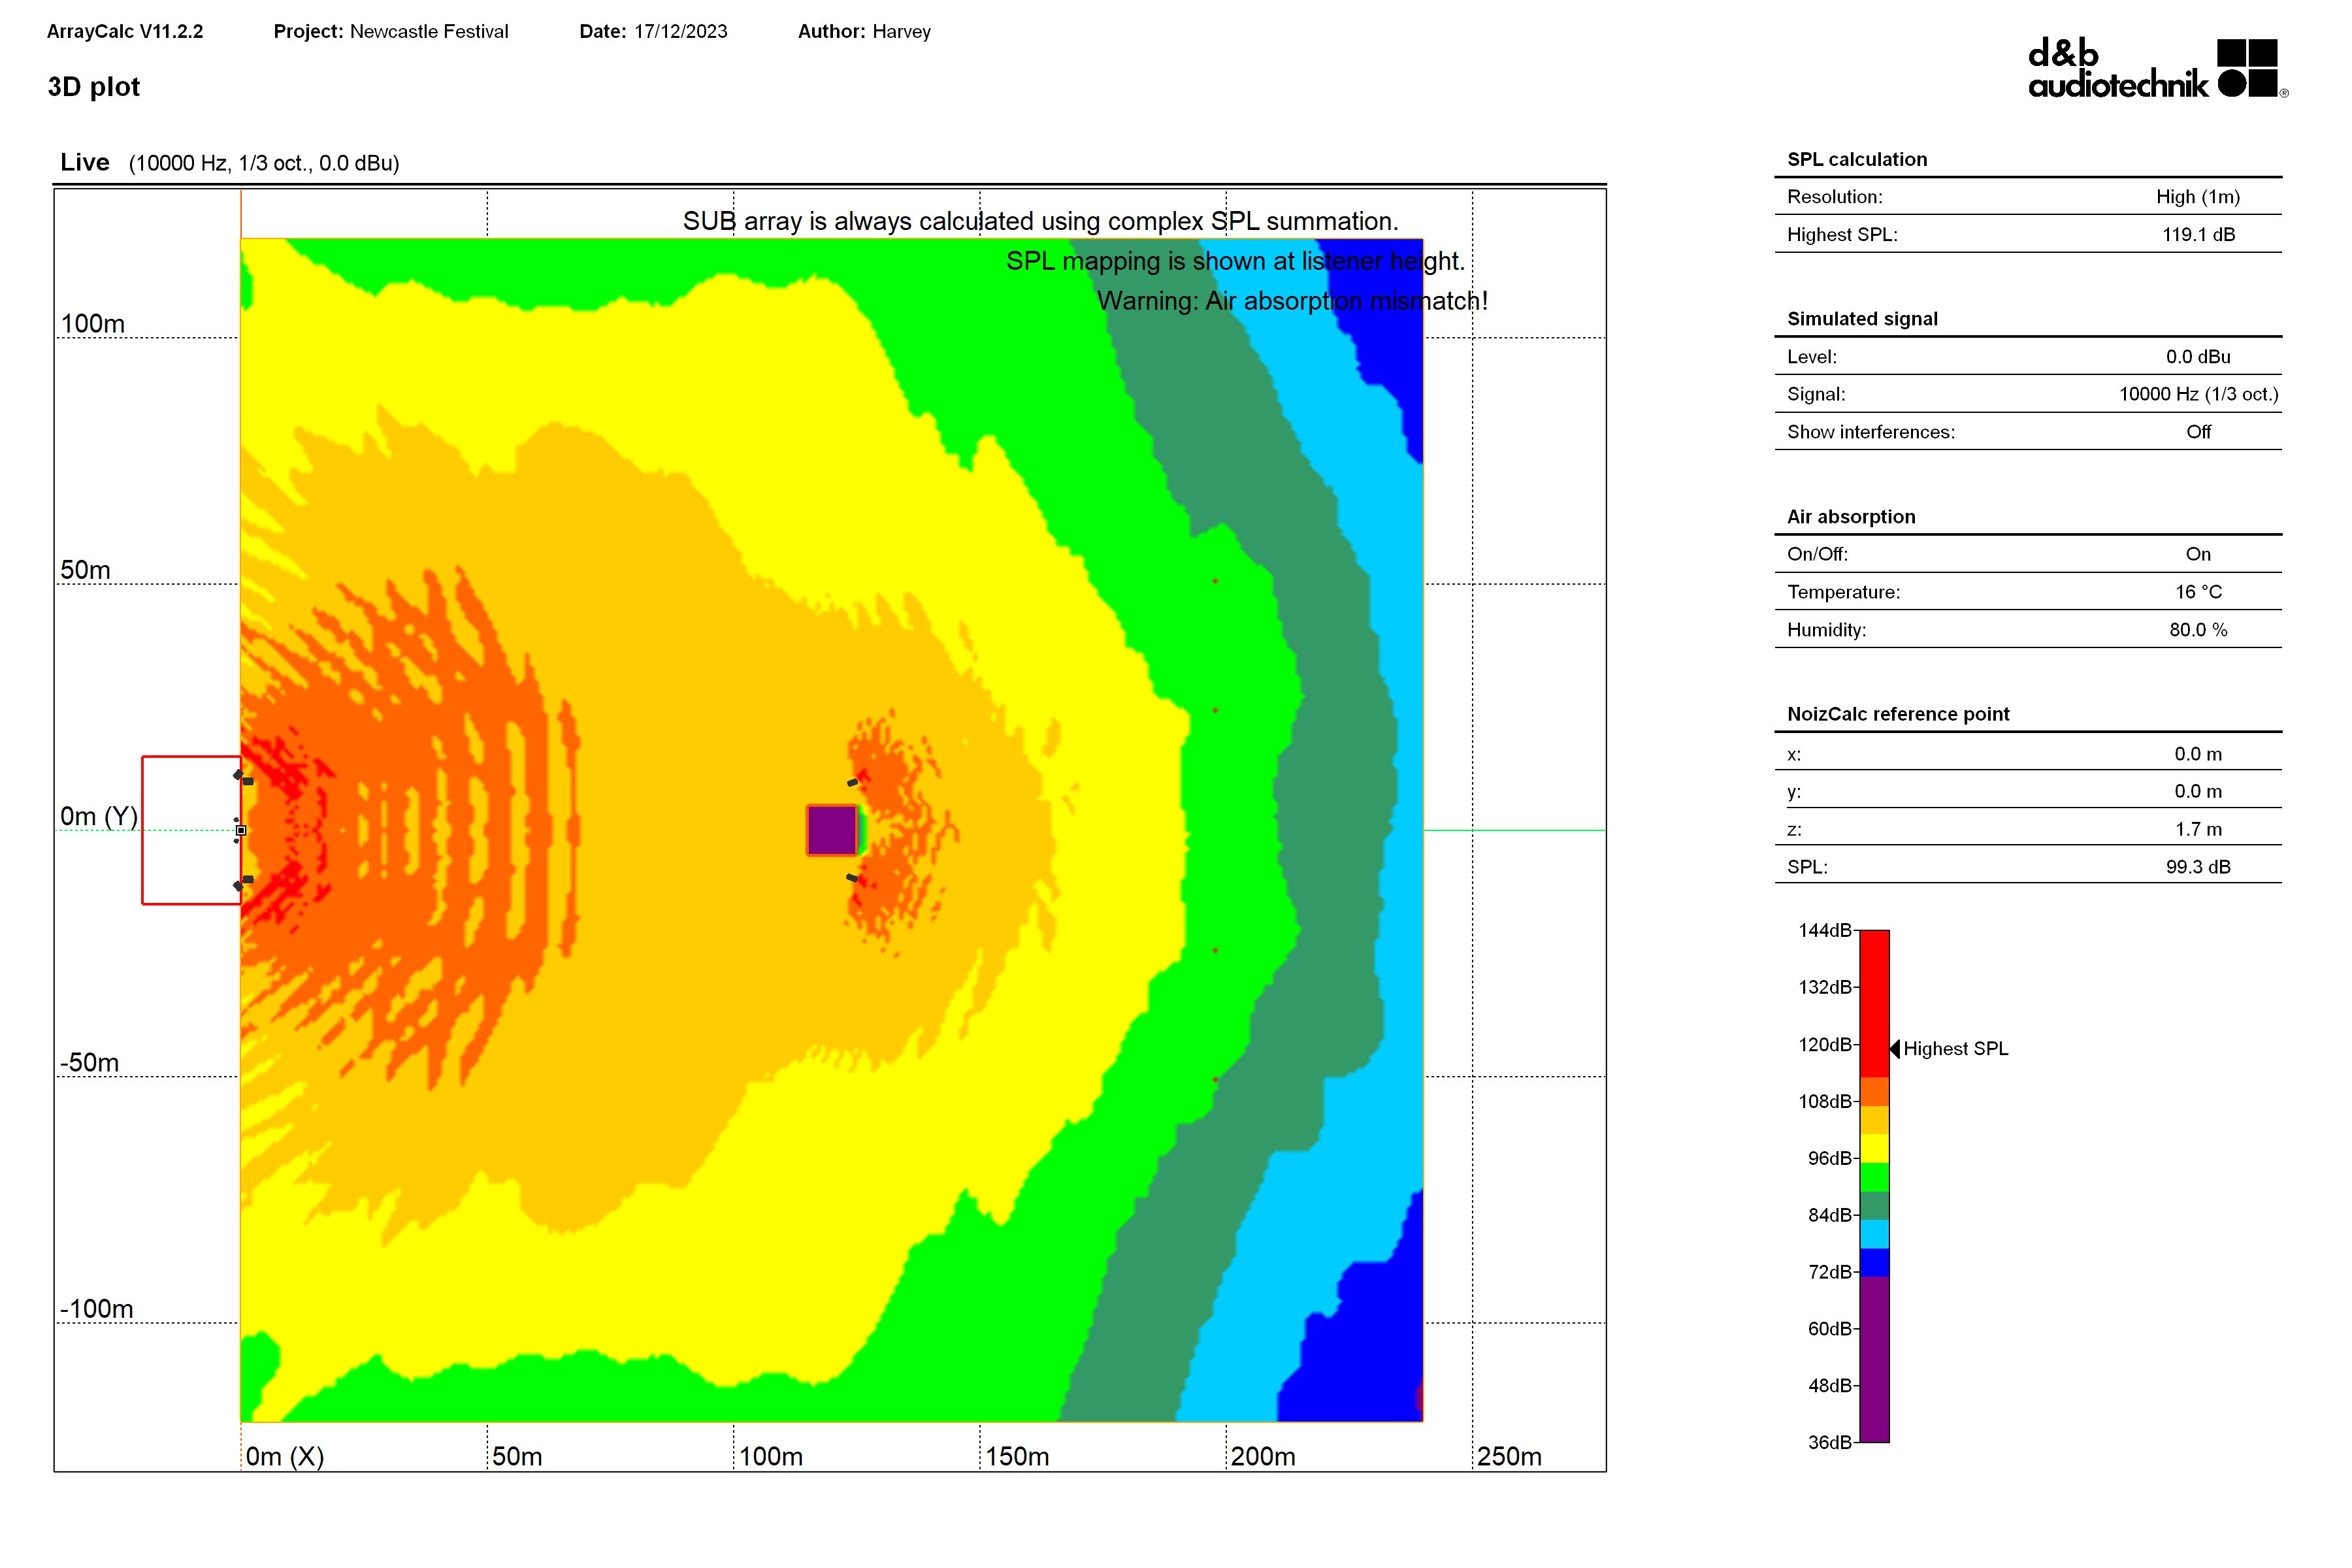
\includegraphics[width=0.5\textwidth]{Images/spl_plot_10khz.png}}      & \multicolumn{1}{c|}{\SI{119.1}{\dB}} & \multicolumn{1}{c|}{\SI{72}{\dB}}  & \multicolumn{1}{c|}{\SI{33.3}{\dB}} & \SI{95.6}{\dB} \\ \hline
            \multicolumn{1}{|c|}{Pink}          & \multicolumn{1}{c|}{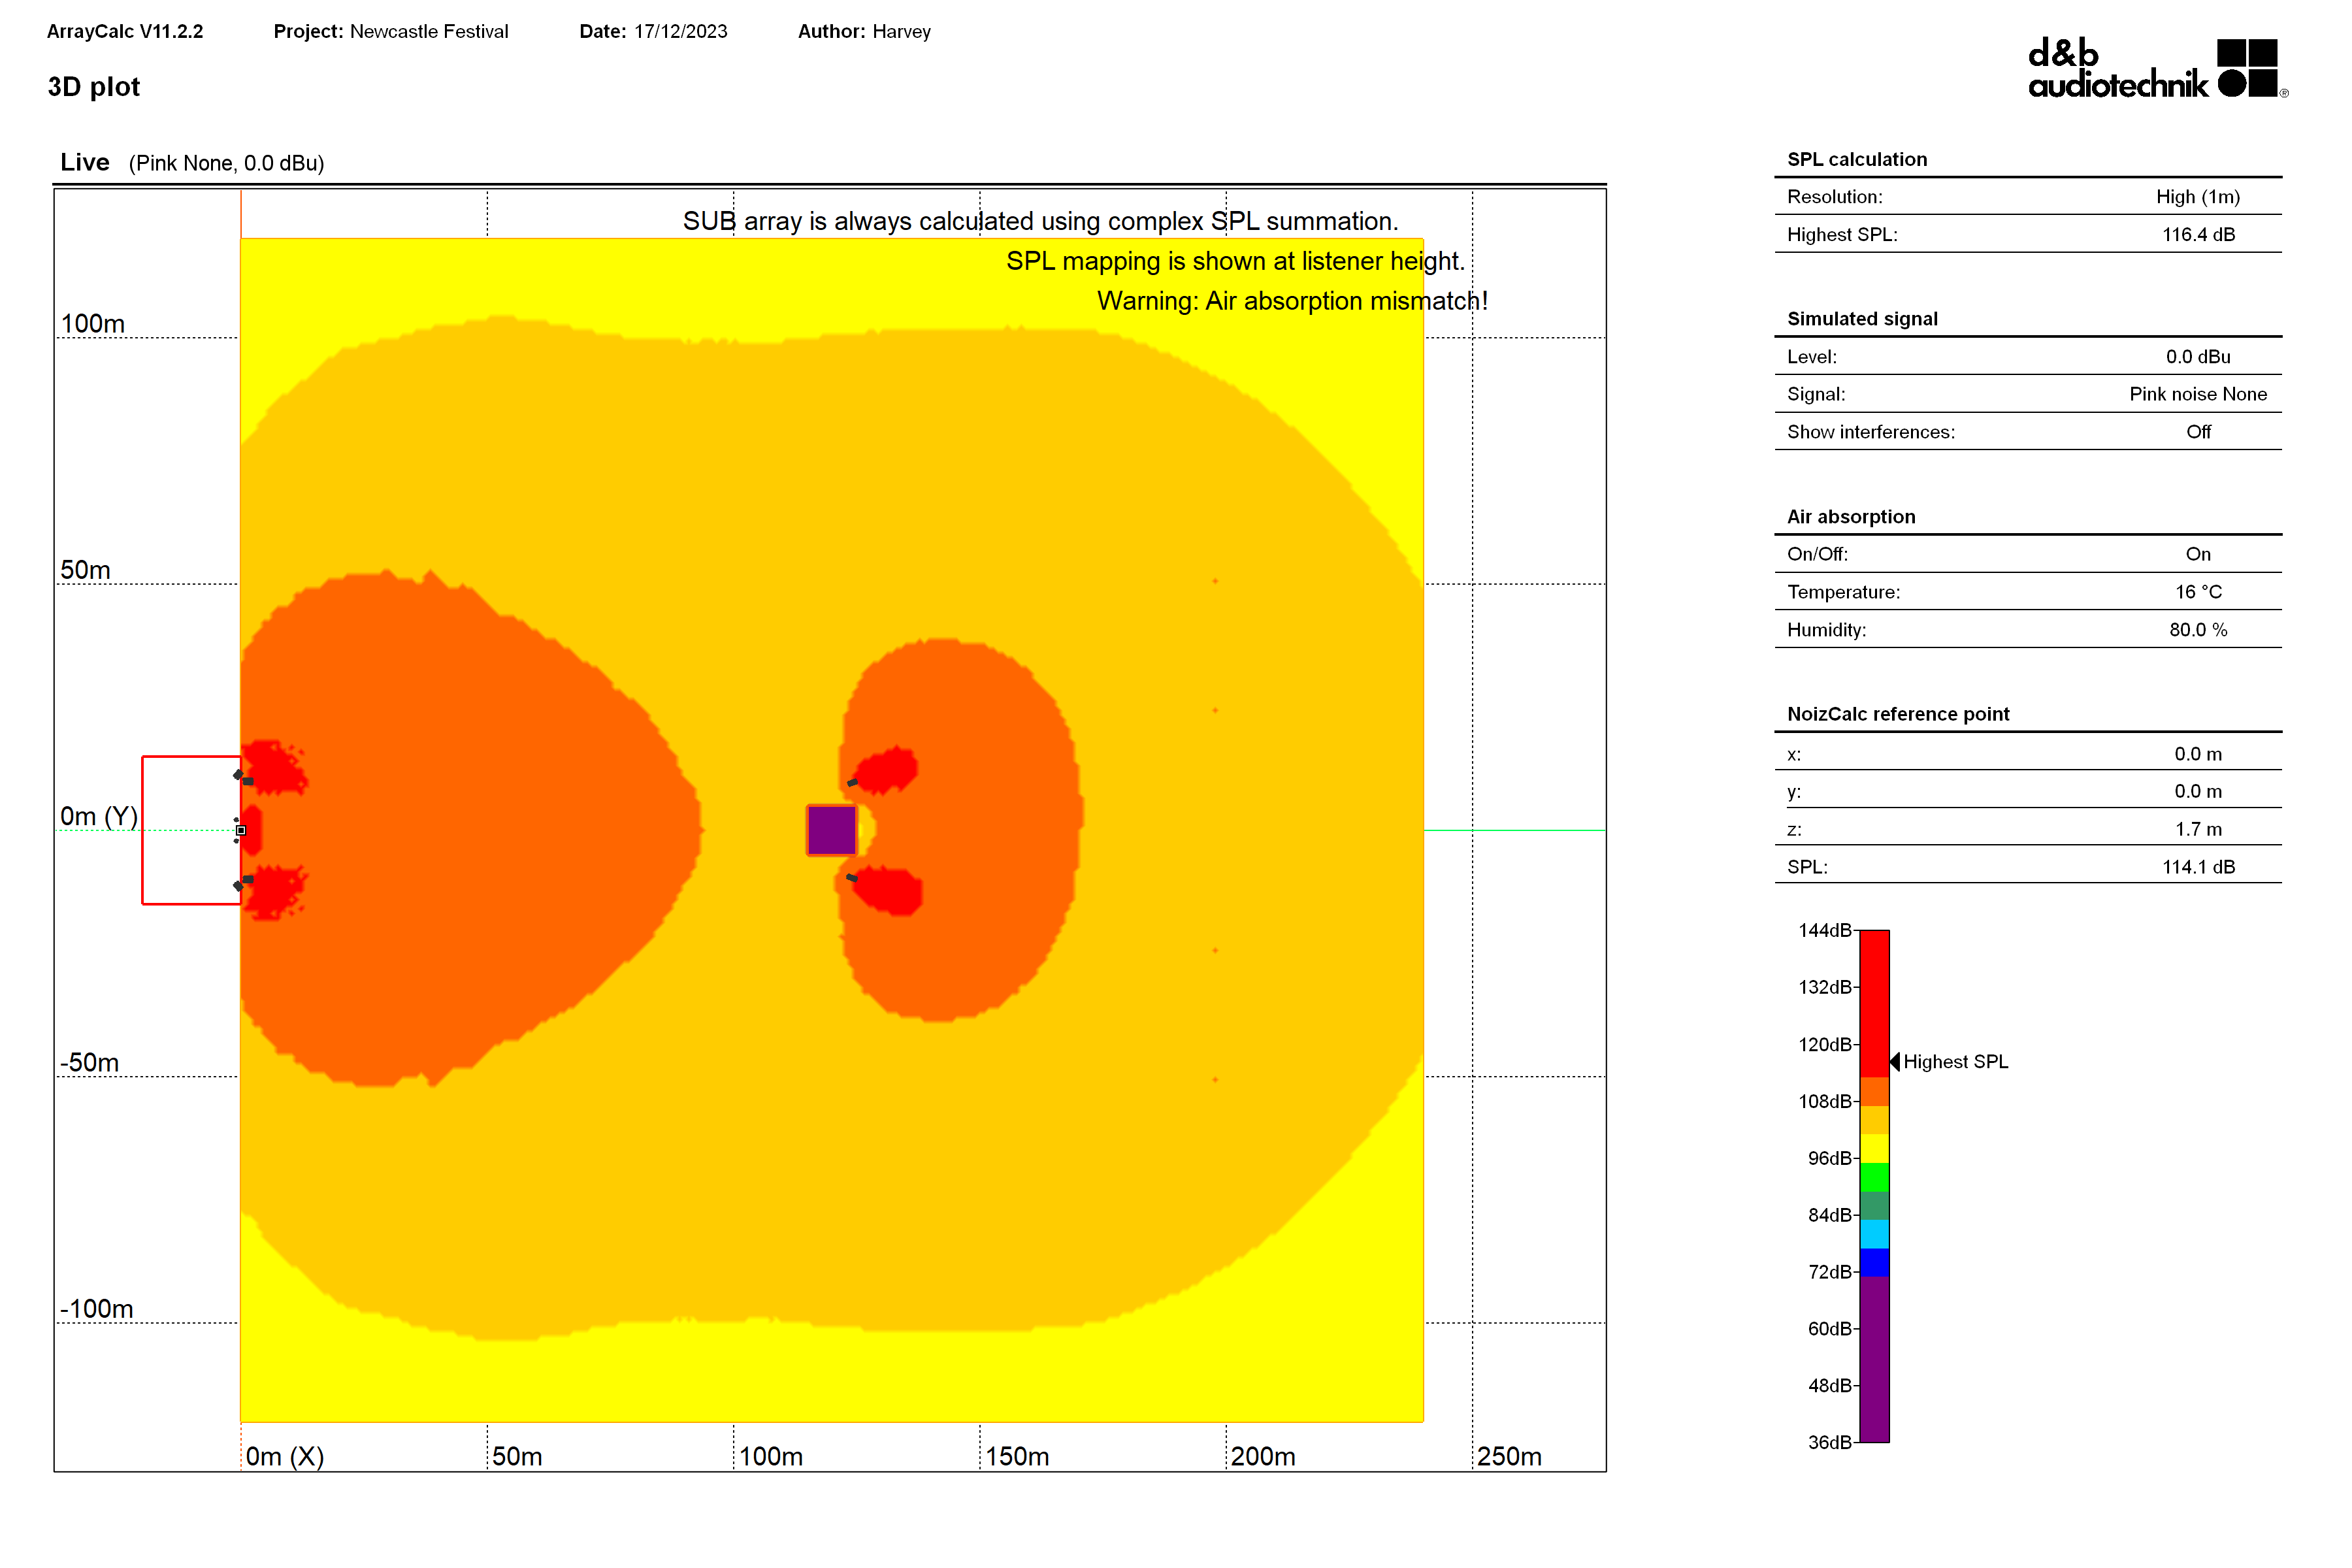
\includegraphics[width=0.5\textwidth]{Images/spl_plot_pink_none.png}}  & \multicolumn{1}{c|}{\SI{116.4}{\dB}} & \multicolumn{1}{c|}{\SI{96}{\dB}}  & \multicolumn{1}{c|}{\SI{14.4}{\dB}} & \SI{106.2}{\dB} \\ \hline
            
            \caption{SPL Mapping}
            \label{tab:spl_mapping}
        \end{longtable}

    \subsubsection{Parts List}
        The parts list for the system is specified in Table \ref{tab:parts_list}.

        \begin{longtable}[H]{|llll|}
            \hline
            \multicolumn{1}{|l|}{\textbf{Origin}} & \multicolumn{1}{l|}{\textbf{d\&b Part no.}} & \multicolumn{1}{l|}{\textbf{Total}} & \textbf{Part name}         \\ \hline
            \endfirsthead
            %
            \endhead
            %
            \multicolumn{4}{|l|}{\textbf{Main}}                                                                                                                    \\ \hline
            \multicolumn{4}{|c|}{GSL}                                                                                                                              \\ \hline
            \multicolumn{1}{|l|}{--}              & \multicolumn{1}{l|}{Z0751}                  & \multicolumn{1}{l|}{44}             & GSL12                      \\ \hline
            \multicolumn{1}{|l|}{--}              & \multicolumn{1}{l|}{Z5706}                  & \multicolumn{1}{l|}{4}              & Hoist chain 4t             \\ \hline
            \multicolumn{1}{|l|}{--}              & \multicolumn{1}{l|}{Z5707}                  & \multicolumn{1}{l|}{2}              & SL Aiming plate (optional) \\ \hline
            \multicolumn{1}{|l|}{--}              & \multicolumn{1}{l|}{Z5708}                  & \multicolumn{1}{l|}{2}              & GSL Flying frame set       \\ \hline
            \multicolumn{4}{|l|}{\textbf{Outfill L}}                                                                                                               \\ \hline
            \multicolumn{4}{|c|}{GSL}                                                                                                                              \\ \hline
            \multicolumn{1}{|l|}{--}              & \multicolumn{1}{l|}{Z0751}                  & \multicolumn{1}{l|}{16}             & GSL12                      \\ \hline
            \multicolumn{1}{|l|}{--}              & \multicolumn{1}{l|}{Z5704}                  & \multicolumn{1}{l|}{1}              & GSL Compression set        \\ \hline
            \multicolumn{1}{|l|}{--}              & \multicolumn{1}{l|}{Z5706}                  & \multicolumn{1}{l|}{2}              & Hoist chain 4t             \\ \hline
            \multicolumn{1}{|l|}{--}              & \multicolumn{1}{l|}{Z5707}                  & \multicolumn{1}{l|}{1}              & SL Aiming plate (optional) \\ \hline
            \multicolumn{1}{|l|}{--}              & \multicolumn{1}{l|}{Z5708}                  & \multicolumn{1}{l|}{1}              & GSL Flying frame set       \\ \hline
            \multicolumn{4}{|l|}{\textbf{Outfill R}}                                                                                                               \\ \hline
            \multicolumn{4}{|c|}{GSL}                                                                                                                              \\ \hline
            \multicolumn{1}{|l|}{--}              & \multicolumn{1}{l|}{Z0751}                  & \multicolumn{1}{l|}{16}             & GSL12                      \\ \hline
            \multicolumn{1}{|l|}{--}              & \multicolumn{1}{l|}{Z5704}                  & \multicolumn{1}{l|}{1}              & GSL Compression set        \\ \hline
            \multicolumn{1}{|l|}{--}              & \multicolumn{1}{l|}{Z5706}                  & \multicolumn{1}{l|}{2}              & Hoist chain 4t             \\ \hline
            \multicolumn{1}{|l|}{--}              & \multicolumn{1}{l|}{Z5707}                  & \multicolumn{1}{l|}{1}              & SL Aiming plate (optional) \\ \hline
            \multicolumn{1}{|l|}{--}              & \multicolumn{1}{l|}{Z5708}                  & \multicolumn{1}{l|}{1}              & GSL Flying frame set       \\ \hline
            \multicolumn{4}{|l|}{\textbf{Delay Array L}}                                                                                                           \\ \hline
            \multicolumn{4}{|c|}{KSL}                                                                                                                              \\ \hline
            \multicolumn{1}{|l|}{--}              & \multicolumn{1}{l|}{Z0781}                  & \multicolumn{1}{l|}{14}             & KSL12                      \\ \hline
            \multicolumn{1}{|l|}{--}              & \multicolumn{1}{l|}{Z0785}                  & \multicolumn{1}{l|}{4}              & KSL-SUB                    \\ \hline
            \multicolumn{1}{|l|}{--}              & \multicolumn{1}{l|}{Z5706}                  & \multicolumn{1}{l|}{2}              & Hoist chain 4t             \\ \hline
            \multicolumn{1}{|l|}{--}              & \multicolumn{1}{l|}{Z5707}                  & \multicolumn{1}{l|}{1}              & SL Aiming plate (optional) \\ \hline
            \multicolumn{1}{|l|}{--}              & \multicolumn{1}{l|}{Z5721}                  & \multicolumn{1}{l|}{1}              & KSL Flying frame set       \\ \hline
            \multicolumn{1}{|l|}{--}              & \multicolumn{1}{l|}{Z5724}                  & \multicolumn{1}{l|}{1}              & KSL Compression set        \\ \hline
            \multicolumn{1}{|l|}{--}              & \multicolumn{1}{l|}{Z5747}                  & \multicolumn{1}{l|}{1}              & KSL-SUB Adapter frame      \\ \hline
            \multicolumn{4}{|l|}{\textbf{Delay Array R}}                                                                                                           \\ \hline
            \multicolumn{4}{|c|}{KSL}                                                                                                                              \\ \hline
            \multicolumn{1}{|l|}{--}              & \multicolumn{1}{l|}{Z0781}                  & \multicolumn{1}{l|}{14}             & KSL12                      \\ \hline
            \multicolumn{1}{|l|}{--}              & \multicolumn{1}{l|}{Z0785}                  & \multicolumn{1}{l|}{4}              & KSL-SUB                    \\ \hline
            \multicolumn{1}{|l|}{--}              & \multicolumn{1}{l|}{Z5706}                  & \multicolumn{1}{l|}{2}              & Hoist chain 4t             \\ \hline
            \multicolumn{1}{|l|}{--}              & \multicolumn{1}{l|}{Z5707}                  & \multicolumn{1}{l|}{1}              & SL Aiming plate (optional) \\ \hline
            \multicolumn{1}{|l|}{--}              & \multicolumn{1}{l|}{Z5721}                  & \multicolumn{1}{l|}{1}              & KSL Flying frame set       \\ \hline
            \multicolumn{1}{|l|}{--}              & \multicolumn{1}{l|}{Z5724}                  & \multicolumn{1}{l|}{1}              & KSL Compression set        \\ \hline
            \multicolumn{1}{|l|}{--}              & \multicolumn{1}{l|}{Z5747}                  & \multicolumn{1}{l|}{1}              & KSL-SUB Adapter frame      \\ \hline
            \multicolumn{4}{|l|}{\textbf{Nearfill Array}}                                                                                                          \\ \hline
            \multicolumn{4}{|c|}{V-Series}                                                                                                                         \\ \hline
            \multicolumn{1}{|l|}{--}              & \multicolumn{1}{l|}{Z0515}                  & \multicolumn{1}{l|}{6}              & V8                         \\ \hline
            \multicolumn{1}{|l|}{--}              & \multicolumn{1}{l|}{Z5380}                  & \multicolumn{1}{l|}{2}              & V Flying frame             \\ \hline
            \multicolumn{4}{|l|}{\textbf{Frontfill}}                                                                                                               \\ \hline
            \multicolumn{4}{|c|}{Y-Series}                                                                                                                         \\ \hline
            \multicolumn{1}{|l|}{--}              & \multicolumn{1}{l|}{Z0703}                  & \multicolumn{1}{l|}{4}              & Y10P                       \\ \hline
            \multicolumn{4}{|l|}{\textbf{SUB array}}                                                                                                               \\ \hline
            \multicolumn{4}{|c|}{KSL}                                                                                                                              \\ \hline
            \multicolumn{4}{|c|}{SL-SUB}                                                                                                                           \\ \hline
            \multicolumn{1}{|l|}{--}              & \multicolumn{1}{l|}{Z0760}                  & \multicolumn{1}{l|}{12}             & SL-SUB                     \\ \hline
            \multicolumn{4}{|l|}{\textbf{Devices}}                                                                                                                 \\ \hline
            \multicolumn{1}{|l|}{--}              & \multicolumn{1}{l|}{Z2710}                  & \multicolumn{1}{l|}{44}             & D80                        \\ \hline
            \multicolumn{1}{|l|}{--}              & \multicolumn{1}{l|}{Z2750}                  & \multicolumn{1}{l|}{4}              & D20                        \\ \hline
            \multicolumn{1}{|l|}{--}              & \multicolumn{1}{l|}{Z2850}                  & \multicolumn{1}{l|}{12}             & D40                        \\ \hline
            \multicolumn{1}{|l|}{--}              & \multicolumn{1}{l|}{Z4010}                  & \multicolumn{1}{l|}{2}              & DS10                       \\ \hline
            \multicolumn{1}{|l|}{--}              & \multicolumn{1}{l|}{Z4100}                  & \multicolumn{1}{l|}{2}              & DS100                      \\ \hline
           
            \caption{Parts List}
            \label{tab:parts_list}
        \end{longtable}

    \subsubsection{Rigging Requirements}
        The full rigging requirements are provided at \ref{appendix:speaker_rigging} with the required pick points, loads and dimensions specified.

    \subsubsection{Delay Times}
        Delays are crucial to ensure proper alignment of multiple audio sources. Especially when arrays are distributed across different locations and distances from the audience. To calculate the necessary delay times for each speaker array, trigonometry is employed to account for the varying distances between the individual speaker hangs.

        The time delay ($t$) needed to time-align two speaker systems with positions ($x_1, y_1, z_1$) and ($x_2, y_2, z_2$) can be calculated using the formula:

        \begin{equation}\label{eq:time_delay}
            t = \frac{\sqrt{(x_2 - x_1)^2 + (y_2 - y_1)^2 + (z_2 - z_1)^2}}{v}
        \end{equation}

        where ($v$) is the speed of sound in air.

        To calculate the speed of sound ($v$), the following formula is used:

        \begin{equation}\label{eq:speed_of_sound}
            v = 331.4 \sqrt{1 + \frac{T}{273.15}} + 0.6 \times H
        \end{equation}

        where ($T$) is the temperature in degrees Celsius, and ($H$) is the relative humidity.
        
        \citet{cramer1993} and \citet{picard2008} demonstrates equations that includes the altitude (Equation \ref{eq:complex_speed_of_sound}). Using the altitude value, the air pressure is calculated with the barometric formula (Equation \ref{eq:barometric_formula}):

        \begin{equation}\label{eq:barometric_formula}
            P = P_0 e^{-\frac{gM(h - h_0)}{RT}}
        \end{equation}
            
        Where:
        \begin{itemize}
            \item $h$ is the altitude at which we want to calculate the pressure, expressed in meters.
            \item $P$ is the air pressure at altitude $h$.
            \item $P_0$ is the pressure at the reference level $h_0$. In our pressure calculator, it is assumed that the reference level is located as sea level, so $h_0 = 0$.
            \item $T$ is the temperature at altitude $h$, expressed in Kelvins. The temperature at altitude calculator may help you find it.
            \item $g$ is the acceleration due to the gravitational force. For Earth, $g = \SI{9.80665}{\m/s\squared}$.
            \item $M$ is the molar mass of air. For Earthly air, $M = \SI{0.0289644}{\kg\mol}$.
            \item $R$ is the universal gas constant. Its value is equal to $R = \SI{8.31432}{N \cdot m/(mol \cdot K)}$.
        \end{itemize}

        This is then applied to \citeauthor{cramer1993}'s formula:

        \begin{equation*}\label{eq:complex_speed_of_sound}
            \begin{aligned}
            ENH &= \pi \cdot 10^{-8}P + 1.00062 + T^2 \cdot 5.6 \cdot 10^{-7} \\
            PSV_1 &= T_k^2 \cdot 1.2378847 \cdot 10^{-5} - 1.9121316 \cdot 10^{-2} \cdot T_k \\
            PSV_2 &= 33.93711047 - 6.3431645 \cdot 10^3 / T_k \\
            PSV &= e^{PSV_1} \cdot e^{PSV_2} \\
            H &= Rh \cdot ENH \cdot \frac{PSV}{P} \\
            X_w &= \frac{H}{100} \\
            X_c &= 400 \cdot 10^{-6} \\
            C_1 &= 0.603055T + 331.5024 - T^2 \cdot 5.28 \cdot 10^{-4} + \\ & \ldots (0.1495874T + 51.471935 - T^2 \cdot 7.82 \cdot 10^{-4}) \cdot X_w \\
            C_2 &= (-1.82 \cdot 10^{-7} + 3.73 \cdot 10^{-8}T - T^2 \cdot 2.93 \cdot 10^{-10})P + \\ & \ldots (-85.20931 - 0.228525T + T^2 \cdot 5.91 \cdot 10^{-5})X_c \\
            C_3 &= X_w^2 \cdot 2.835149 + P^2 \cdot 2.15 \cdot 10^{-13} - X_c^2 \cdot 29.179762 - 4.86 \cdot 10^{-4}X_wPX_c \\
            C &= C_1 + C_2 - C_3
            \end{aligned}
        \end{equation*}

        Where:
        \begin{itemize}
            \item $Rh$: is the relative humidity.
            \item $Tk$: is the measured ambient temperature in kelvins.
            \item $ENH$: is the molecular concentration of water vapour calculated from $Rh$. Using Giacomo's methods as demonstrated by \citeauthor{rasmussen1997}.
            \item $PSV$ values: are constants taken from \citeauthor{cramer1993}'s equations.
            \item $H$: is the molecular concentration of water vapour.
            \item $Xw$: is the mole fraction of carbon dioxide and water vapour, respectively.
            \item $C$ values: are the speed calculated using the method of \citeauthor{cramer1993} from JASA vol 93 page 2510
        \end{itemize}
        
        Referring to weather averages for Newcastle upon Tyne in July, the temperature typically ranges between 19°C and 13°C, with humidity averaging around 75\% \citep{worldweatheronline2023}.

        Table \ref{tab:delay_times} displays the approximate delay compensations for each source, where the delay reference point is at $X=\SI{150}{\metre}, Y=\SI{0}{\metre}$. These may differ to the ArrayCalc times as phase is also considered to closely align with the subs at specific frequencies as shown in Figure \ref{fig:delay_alignment}. The supporting calculations are provided in the 'DelayAlignTimes' excel file.

        \begin{longtable}[c]{|lllll|}
            \hline
            \multicolumn{5}{|l|}{Temperature = \SI{16}{\celsius}, Humidity = 75\%, Altitude = \SI{64}{\metre}} \\ \hline
            \endfirsthead
            %
            \endhead
            %
            \multicolumn{1}{|l|}{\textbf{Source}} & \multicolumn{1}{l|}{\textbf{X}} & \multicolumn{1}{l|}{\textbf{Y}} & \multicolumn{1}{l|}{\textbf{Z}} & \textbf{Total Delay} \\ \hline
            \multicolumn{1}{|l|}{Delay} & \multicolumn{1}{l|}{\SI{125}{\metre}} & \multicolumn{1}{l|}{\SI{10}{\metre}} & \multicolumn{1}{l|}{\SI{10.5}{\metre}} & \multicolumn{1}{l|}{\SI{364.39}{\ms}} \\ \hline
            \multicolumn{1}{|l|}{Main} & \multicolumn{1}{l|}{\SI{2.4}{\metre}} & \multicolumn{1}{l|}{\SI{10}{\metre}} & \multicolumn{1}{l|}{\SI{12}{\metre}} & \multicolumn{1}{l|}{\SI{13.34}{\ms}} \\ \hline
            \multicolumn{1}{|l|}{Outfill} & \multicolumn{1}{l|}{\SI{0}{\metre}} & \multicolumn{1}{l|}{\SI{12}{\metre}} & \multicolumn{1}{l|}{\SI{10.5}{\metre}} & \multicolumn{1}{l|}{\SI{6.20}{\ms}} \\ \hline
            \multicolumn{1}{|l|}{Sub} & \multicolumn{1}{l|}{\SI{0}{\metre}} & \multicolumn{1}{l|}{\SI{0}{\metre}} & \multicolumn{1}{l|}{\SI{0}{\metre}} & \multicolumn{1}{l|}{\SI{8.33}{\ms}} \\ \hline
            \multicolumn{1}{|l|}{Nearfill} & \multicolumn{1}{l|}{\SI{-0.6}{\metre}} & \multicolumn{1}{l|}{\SI{2.20}{\metre}} & \multicolumn{1}{l|}{\SI{2.5}{\metre}} & \multicolumn{1}{l|}{\SI{6.55}{\ms}} \\ \hline
            \multicolumn{1}{|l|}{Frontfill} & \multicolumn{1}{l|}{\SI{0}{\metre}} & \multicolumn{1}{l|}{\SI{0}{\metre}} & \multicolumn{1}{l|}{\SI{0}{\metre}} & \multicolumn{1}{l|}{\SI{8.33}{\ms}} \\ \hline

            \caption{Delay Times}
            \label{tab:delay_times}
        \end{longtable}

        \begin{figure}[H]
            \centering
            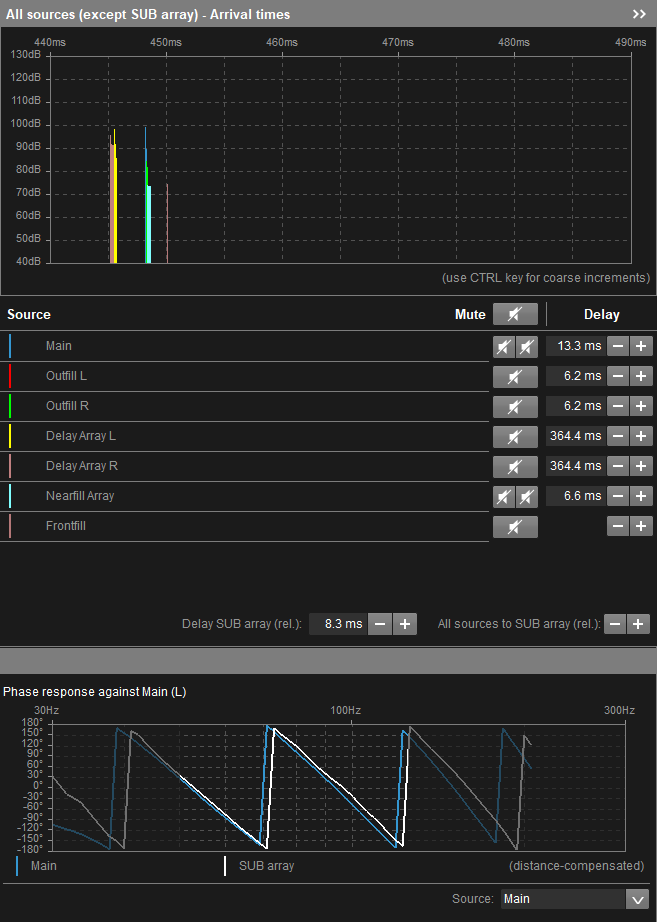
\includegraphics{Images/delay_alignment.png}
            \caption{Time and phase alignment of sources}
            \label{fig:delay_alignment}
        \end{figure}

        \ref{appendix:speaker_delays}

    \subsubsection{Power Requirements}
        a
    
    \subsection{System Selection}
        \subsubsection{Design Considerations}
        \note{Noisecalc here}

        \subsubsection{Signal Engine}
            Using a signal engine such as the DN100 enables compatibility with dante and d\&b's en-space software. En-space can be used to enhance the auditory experience through boundary plane emulation technology \citep{ds100}. This unit will be configured in redundancy mode within the dante network.

    \subsection{System Integration}
        \note{Add diagram routing here}

        The amplifier configurations are provided at \ref{appendix:speaker_amp_config} and the full patch sheet for the sound system is displayed at \ref{appendix:speaker_patch}; showing the routing between the network bridges, signal engine, amplifiers, and speakers.

        \subsubsection{Audio Networking}
        \note{add dante stuff here}
        